In its most general form, the $k$-List problem is defined as follows:
\begin{definition}[$k$-List Problem] \label{def:kList}
	Given $k$ lists $L_1, \ldots, L_k$ of elements from a set $X$, the task is to find $k$-tuples $(x_1, \ldots, x_k) \in L_1 \times \ldots \times L_k$ that satisfy some condition $C$. Such a tuple $(x_1, \ldots, x_k)$ is called a solution to the $k$-List problem.
\end{definition}

Typically, the elements of the lists are iid.\ uniformly chosen from $X$, and the size of the lists $L_i$ is exponential in the bit-length of a list-element. The number of output solutions depends on a concrete instantiation of the $k$-List problem: in some cases (as in Sect.~\ref{sec:Approx_kList_Euclid}), we require to output almost all solutions, while sometimes only one or constant number of solutions is enough. 

In the examples of the $k$-List problem we consider here, a set $X$ from where the list-elements are taken, is equipped with a metric. For instance, in case $X = \ZO{n}$ it is the Hamming weight (i.e., distance from $\zerovec$) $wt(\cdot)$, and in case $X$ is a subspace of Euclidean space, there is the $\ell_2$-norm defined on $X$. Condition $C$ that must be satisfied by the output will be naturally related to this metric. For example, when $L_i \subset \R^n$, we can ask for tuples whose sum, $\xvec_1 + \ldots + \xvec_k$, is short. We give more examples below.

Clearly, algorithms for $k$-List problems require at least $\sum_i |L_i|$ memory, and the running time is at least $\max\{\sum_i |L_i|, \# \text{output solutions}\}$. We also consider cases when lists are equal. 
 
There is a plethora of cryptographic tasks that can be phrased as a $k$-List problem. Probably the most popular is the collision-search problem for a hash-function $f:\ZO{*} \rightarrow \ZO{n}$. The birthday paradox states that if we have 2 lists each of size $2^{n/2}$ with elements of the form $(x, f(x))$ in the first list and $(x', f(x'))$ in the second, then search for a pair with s.t.\ $f(x)=f(x')$ gives a collision for $f$ with constant success probability.


Wagner extended this idea to what he calls the Generalized Birthday problem \cite{C:Wagner02}: given $k$ lists $L_i \subset \ZO{n}$, a tuple $(\xvec_1, \ldots, \xvec_k) \in L_1 \times \ldots \times L_k$ is a solution if $\xvec_1 \oplus \ldots \oplus \xvec = \tvec$ for some input $\tvec \in \ZO{n}$. He proposed an algorithm running in time $\xTLandau(2^{\sqrt{n}})$ that uses $\xTLandau(2^{\sqrt{n}})$ lists of size $\xTLandau(2^{\sqrt{n}})$. The Generalized Birthday problem has found its applications in breaking hash-functions, forging signature schemes \cite{C:Wagner02}, and attacking stream-ciphers \cite{AC:NikSas15}.

Another famous $k$-List algorithm is due to Blum, Kalai, and Wasserman \cite{BKW}. We write \BKW when we refer to this algorithm. It solves the \emph{Learning Parity with Noise} problem -- a binary counterpart of $\LWE$ -- a very well-known problem in machine learning. Different to \LWE, the vectors $\avec_i$ and the secret $\svec$ are now from $\ZO{n}$, and the noise $e_i$ follows the Bernoulli distribution with parameter $\tau \in [0, 1/2)$. In contrast to Wagner's algorithm, where the list-sizes and their number $k$ can be optimally chosen, the number of lists in the \BKW algorithm is limited to $n^{1-\eps}$. A tuple $(\xvec_1, \ldots, \xvec_k)$ is a solution if $wt(x_1 \oplus \ldots \oplus x_k) = 1$. 

The \BKW algorithm received even more attention after Albrecht et al.\ in \cite{DCC:ACFFP15} analyzed it for \LWE. In this case, the list elements are formed from $\avec_i \in \Z_q^n$ -- the first components of \LWE samples. A tuple we seek for must satisfy $\xvec_1 + \ldots + \xvec_k =  (0, \ldots 0, 1, 0, \ldots, 0) \bmod q$. Recently, Kircher-Fouque \cite{C:KirFou15} and Guo et al.\ \cite{C:GuoJohSta15} independently realized that the condition can be slightly relaxed: asking for a tuple with a short sum $\xvec_1 + \ldots + \xvec_k$ leads to an improved algorithm for \LWE. %For both, \LWE and \LPN problems, the input lists $L_i$ are identical.

Kuperberg's quantum algorithm for the Dihedral Hidden Subgroup problem \cite{Kup05} is yet another example of a $k$-List algorithm. It operates with lists $L_i \subset \Z_N$ and searches for a tuple $(x_1, \ldots, x_k)$ that sums up to $N/2$. This is a quantum analog of Wagner's algorithm for the Generalized Birthday problem, but it operates with relative phases, $x_i$'s, of quantum superpositions. Optimal list sizes and $k$ are chosen exactly in the same way as in Wagner's algorithm. 

If we turn our attention to $k$-List problems over Euclidean spaces, we land in the realm of algorithms for the Shortest Vector Problem. Namely, for \ $X \subset \Lat$, and $k=2$, the task of finding pairs $(\xvec_1, \xvec_2) \in L_1 \times L_2$ s.t.\ $\| \xvec_1 + \xvec_2 \| < \min \{ \| \xvec_1 \|, \| \xvec_2 \| \}$ is at heart of so-called \emph{sieving} algorithms for \SVP \cite{STOC:AjtKumSiv01}. List-elements are vectors of a lattice. The lists are \emph{exponential} in the lattice-dimension. An important requirement here is that the number of solutions has to be asymptotically equal to the size of input lists, i.e.\ exponential. 
Large memory complexity precludes sieving algorithms from being practically competitive with other algorithms for \SVP.

A progress towards memory-efficient \SVP-sieving was recently achieved by Bai, Laarhoven, and Stehl\'{e} (BLS, for short). In \cite{BLS16}, they generalize sieving algorithms for $k$ larger than 2. Intuitively, the larger $k$ is, the shorter the input lists can be to guarantee the same number of solutions, since instead of $|L_1| \cdot |L_2|$ tuples, we have $|L_1| \cdot \ldots \cdot |L_k|$ tuples in total. On the other hand, larger $k$ results in increased running time. In Sect.~\ref{sec:Approx_kList_Euclid} we present a $k$-List algorithm that achieves a better running time than the one presented in \cite{BLS16}.

We should stress that in all these examples the expected number of solutions is very large. In other words, $k$-List problems are \emph{high density} problems. The algorithms exploit this fact by dropping many solutions and focusing only on solutions with some distinguished property. 

A common strategy to solve a $k$-List problem is to identify such a distinguished property (or a search criterion) for a solution-tuple that would help to find a solution. The size of input lists is then chosen such that the number of solutions that satisfy this property is large enough.

For example, Wagner's algorithm \cite{C:Wagner02} outputs a solution $(\xvec_1, \ldots, \xvec_n)$ if $[(\xvec_i \oplus \xvec_{i+1})]_{1}^{\ell} = \zerovec$ for all odd $i<n$, where for a vector $\xvec$ we denote $[x]_i^j$ as its projection on coordinates $(i, \ldots j)$ for $i \leq j$. The value $\ell$  in Wanger's algorithm is optimally chosen as $\ell = \sqrt{n}$. Such a pair-wise constraint allows to search for a pair of vectors $(\xvec_i, \xvec_{i+1}) \in L_i \times L_{i+1}$ independently from another pair $(\xvec_j, \xvec_{j+1}) \times (L_j, L_{j+1})$. Each of these pairs is then combined into a vector producing two new lists with elements having 0's on the last $\ell$ coordinates. The same constraint is then put on the next $\ell$ coordinates of vectors from the new lists. Of course, with this approach we lose many solutions and we account for that by appropriately setting the input-lists' sizes. Currently, the searching criteria of Wagner's algorithm is the best for the Generalized $k$-List problem over $\ZO{n}$.

We describe our searching criteria in Sect.~\ref{subsec:ConfigL2} for \SVP. It is similar to Wagner's criteria in a sense that it puts a \emph{pairwise} constraint on a solution-tuple. On the other hand, different from Wagner's algorithm, our constraint makes a `global' effect on all the lists: choosing $\xvec \in L_1$ affects not only $L_2$, but all $L_i$'s. It turns out that our constraint does not only speed up the search, but is also met by a large fraction of all the solutions. Thus, our searching constraint does not incur an growth of the input lists. This is particularly beneficial for \SVP-sieving where memory is a big concern.  

Finally, in Sect.~\ref{sec:ApproxQary}, we present another $k$-List algorithm but now for the 
\emph{approximate} \SVP problem on $q$-ary lattices of dimension $2n$, where the approximation factor is $\poly(n)$. We present two algorithms: the first is very similar to the \BKW algorithm presented in \cite{C:GuoJohSta15, C:KirFou15}. The second puts a more rigid constraint on the solution-tuple, which nevertheless, does not increase the input lists and yet results in a faster $k$-List algorithm. 

Table~\ref{table:kListAlgs} summarizes known $k$-List algorithms. 



\clearpage

\renewcommand{\arraystretch}{1.6}
\begin{table}[h]
\centering
	\resizebox{\textwidth}{!}{%
	\begin{tabular}{|l | c | c | c |}
		\hline
			\multicolumn{4}{|c|}{$L_i \subset \ZO{n}$} \\ \hline 
			\multicolumn{1}{|c|}{Algorithm} &  $k$ & $| L_i |$ & $T$ \\ \hline
			$\BKW$ for \LPN: & & & \\
			\hspace{3pt} $ wt(\xvec_1 \oplus \ldots \oplus \xvec_k) = 1$ (\cite{BKW}), or &  &  & \\ 
			\hspace{3pt}  $wt(\xvec_1 \oplus \ldots \oplus \xvec_k)$ - small (\cite{AC:GuoJohLon14}) & & & \\  %\cline{2-4}
			\hspace{15pt} $\bullet$ $2^{\bigO(\tfrac{n}{\log n})}$ samples & $n^{1-\eps}$ & $2^{\bigO(\frac{n}{\log n})}$ & $2^{\bigO(\frac{n}{\log n})}$ \\ \cline{2-4}
			\hspace{15pt} $\bullet$ $\poly(n)$ samples \cite{LyuLPN05} &$n^{1-\eps}$ &  $\poly(n)$ &  $2^{\bigO(\frac{n}{\log \log n})}$ \\ \hline 
			Wagner's $k$-tree algorithm \cite{C:Wagner02} & \multirow{2}{*}{$k$} &  \multirow{2}{*}{$\softO(k2^{\frac{n}{\log k +1}})$} & \multirow{2}{*}{$\softO(k2^{\frac{n}{\log k +1}})$} \\ 
			\hspace{3pt} $\xvec_1 \oplus \ldots \oplus \xvec_k = \tvec$ for some input $\tvec$ &  &  & \\ \hline
			Extended $k$-tree algorithm  \cite{SODA:MinSin09}  & \multirow{2}{*}{$k$} & \multirow{2}{*}{$m$} & \multirow{2}{*}{\parbox[t]{4cm}{ $2^{(\log k + \frac{n-2^p \log m}{\log k -p})}$, \linebreak \scriptsize where $p$ is the smallest integer s.t.\ $n \leq (\log k -p +1)2^p \log m$ } } \\
			\hspace{3pt} $\xvec_1 \oplus \ldots \oplus \xvec_k = \tvec$ for some input $\tvec$ &  &  & \\ \hline 
			\multicolumn{4}{|c|}{$L_i \subset \Z_q$} \\ \hline 
			Dense Subset-Sum \cite{Lyu05} & \multirow{2}{*}{ $\tfrac{1}{2} n ^{1-\eps}$} & \multirow{2}{*}{$2^{\bigO(\tfrac{n^{\eps}}{\log n})}$} &  \multirow{2}{*}{$2^{\bigO(\tfrac{n^{\eps}}{\log n})}$} \\ 
			\hspace{3pt} $\sum_{i \in I} x_i = t \bmod q$, $q = 2^{n^{\eps}}$ & & & \\ \hline
			Kuperberg's algorithm \cite{Kup05}  & \multirow{2}{*}{$2^{\bigO(\sqrt{n})}$}  & \multirow{2}{*}{$2^{\bigO(\sqrt{n})}$} & \multirow{2}{*}{$2^{\bigO(\sqrt{n})}$} \\ 
			\hspace{3pt} $\sum_{i \in I} x_i = q/2$, $q = 2^n$  & & & \\ \hline 
			\multicolumn{4}{|c|}{$L_i \subset \Z_q^n$} \\ \hline
			$\BKW$ for \LWE with parameters $(n, \alpha, q)$: & & & \\
				\hspace{5pt} $\bullet$ $2^{\TLandau(n)}$ \LWE samples  & & & \\ 
				\hspace{15pt} -- $\| \xvec_1 + \ldots + \xvec_k \| = 1$ \cite{DCC:ACFFP15} & $\TLandau(n)$ & $2^{\frac{1}{2} \frac{\cq}{\ca - 1/2}n + \smallo(n) }$ & $2^{\frac{1}{2} \frac{\cq}{\ca - 1/2}n + \smallo(n) }$ \\ %\cline{2-4}
				\hspace{15pt} -- $\| \xvec_1 + \ldots + \xvec_k \|$ - small \cite{C:GuoJohSta15, C:KirFou15} & $\TLandau(n)$ & $2^{\frac{\cq}{1+2 \ln(\cq / (\cq+\ca))} n + \smallo(n)}$ & $2^{\frac{\cq}{1+2 \ln(\cq / (\cq+\ca))} n + \smallo(n)}$  \\ %\cline{2-4}
				\hspace{5pt} $\bullet$ $\TLandau(n \log n)$ \LWE samples & & & \\
				\hspace{15pt} -- $\| \xvec_1 + \ldots + \xvec_k \| = 1$ & $\TLandau(n)$ & $\TLandau(n \log n)$ & $2^{\frac{1}{2} \frac{\cq}{\ca} n + \smallo(n) }$ \\
				\hspace{15pt} -- $\| \xvec_1 + \ldots + \xvec_k \|$ - small \cite{DCC:HKM} & $\TLandau(n)$ & $\TLandau(n \log n)$ & $2^{\frac{1}{\ln(\cq / (\cq+\ca))} n + \smallo(n)}$ \\  \hline  
			\multicolumn{4}{|c|}{$L_i \subset \Lat$} \\ \hline 
			Sieving algorithms for \SVP &  & & \\ 
			\hspace{3pt} $\bullet$ $\| \xvec_1 \pm \xvec_2 \| < \max\{ \| \xvec_1 \|, \| \xvec_2 \| \}$ \cite{SODA:BDGL16} & 2 & $2^{0.208n + \smallo(n)}$ & $2^{0.292n + \smallo(n)}$ \\
			\hspace{3pt} $\bullet$ $\| \xvec_1 \pm \xvec_2 \pm \ldots \pm \xvec_k \| < \max_i\{ \| \xvec_i \| \}$ & & & \\ 
			\hspace{15pt} -- BLS Algorithm \cite{BLS16} & $\Theta(1)$ & \multirow{2}{*}{$\softO \Bigl( \Bigl( \frac{k^{\tfrac{k}{k-1}}}{k+1} \Bigr)^{\tfrac{n}{2}} \Bigr)$} & see Eq.~\eqref{eq:RunTime} \\
			\hspace{15pt} -- Our Algorithm~\ref{alg:AlgConfig} (Sect.~\ref{subsec:KListAlgL2}) & $\Theta(1)$ &  & see Eq.~\eqref{eq:RunTimeBLS} \\ \hline
			\multicolumn{4}{|c|}{$L_i \subset \qLATTp(\AMat) \subset \Z_q^{2n}$} \\ \hline
			Combinatorial algorithms for $\appSVP$ &  & \multicolumn{2}{c|}{} \\ 
			\hspace{3pt} $\| \sum_i \xvec_i \| < n^{\cg} \lambda_1(\qLATTp(\AMat))$, $\cg=\TLandau(1)$ &  &  \multicolumn{2}{c|}{} \\
			\hspace{3pt} $\bullet$ Algorithm~\ref{alg:ApproxSVP} (Sect.~\ref{subsec:qAryAlg}) & $\TLandau(n)$ & \multicolumn{2}{c|}{See Eq.~(\ref{eq:AppSVPRT})} \\
			\hspace{3pt} $\bullet$ Algorithm~\ref{alg:ApproxSVP} (Sect.~\ref{subsec:qAryAlg}) & $\TLandau(n)$ & \multicolumn{2}{c|}{See Eq.~(\ref{eq:AppSVPImprovedRT})} \\
			\hline
	\end{tabular}
	}
	\caption[$k$-List algorithms]{$k$-List algorithms. In the left-most column alongside with an algorithm, we show the condition that should be met by a solution tuple $(x_1, \ldots, x_k)$. For \LWE, we set $q = n^{\cq}, \alpha = \frac{1}{n^{\ca}}$.
	\label{table:kListAlgs}}
\end{table}

\clearpage

\section{Approximate $k$-List in Euclidean norm} \label{sec:Approx_kList_Euclid}

The problem we are going solve in this section is the following special case of the $k$-List problem. This problem is at the heart of sieving algorithms for the Shortest Vector Problem.


\begin{definition}[Approximate $k$-List problem in $l_2$-norm] \label{def:kListL2}
Let $0 < t < \sqrt{k}$. Given $k$ lists $L_1, \ldots, L_k$ of equal exponential size whose elements are iid.\ uniformly chosen vectors from the $n$-sphere $\Sphere{n}$, the task is to output a $1-\smallo(1)$-fraction of $k$-tuples $\xvec_1 \in L_1, \ldots, \xvec_k \in L_k$ s.t.\ $\|\xvec_1 + \ldots + \xvec_k \|^2 \leq t^2$. Such a tuple $(\xvec_1, \ldots, \xvec_k)$ is called a solution to the approximate $k$-List problem. 
\end{definition}

We analyze the case where $t$ and $k$ are constant and the input lists are of size $2^{\const n}$ for some constant $\const$. The restriction $t < \sqrt{k}$ is set to get a meaningful problem. Due to the fact that for large $n$, random vectors $\xvec_i$'s from $\Sphere{n}$ are almost orthogonal with high probability (cf.\ Thm.~\ref{thm:WishartDist}), a $1-\smallo(1)$-fraction of tuples $(\xvec_1, \ldots, \xvec_k) \in L_1 \times \ldots \times L_k$ satisfy $\| \xvec_1 + \ldots + \xvec_k \|^2 \approx k$. So the problem is non-trivial when either $t< \sqrt{k}$, or $t>\sqrt{k}$. We concentrate on the former. With a simple modification our results apply to the latter case as well. Moreover, our algorithm works for lists of different sizes, but it would unnecessarily complicate the analysis, so we stick to lists of equal size. Additionally, equally-sized lists is a relevant scenario for the \SVP-sieving algorithms.

In the applications to sieving (see Sect.~\ref{subsec:ApproxSVP}), we have $t=1$ and look for solutions with the property $\|\xvec_1 \pm \ldots \pm \xvec_2 \| \leq 1$. Since there are $2^k  = \bigO(1)$ possible choices for signs, we can consider each choice separately increasing the running time of the algorithm by a constant factor. %It leads to few optimizations considered in Sect.~\ref{subsec:KListResults}, but they do not change the asymptotics.

\subsection{Configurations} \label{subsec:ConfigL2}

All the $k$-List algorithms make use of the fact that there are many solution-tuples and we are allowed to output a fraction of all the solutions. 
The main challenge in designing an efficient $k$-List algorithm is to identify a criterion s.t.\ (1) a solution that matches the criterion is easy to find, and (2) enough solutions satisfy this criterion.  The first property leads to a faster algorithm, the second is specified by the problem. In the case of the approximate $k$-List problem, we want to output almost all solutions.

To define the criterion we use in our algorithm, recall the definition of a Gram matrix.

\begin{definition}[Gram Matrix]
 For vectors $\xvec_1, \ldots, \xvec_k$ from $\R^n$, the \emph{Gram matrix} $C \in \R^{k \times k}$ is a positive semidefinite matrix whose entries are pairwise inner products: $C_{i, j} = \ScProd{x_i}{x_j}$.
\end{definition}  

Note that the Gram matrix is invariant under simultaneous rotations and reflections of all $\xvec_i$'s. This property also holds for a $k$-tuple from $\Sphere{n}$ that forms a solution to the approximate $k$-List problem as both, rotation and reflection, preserve distance. Hence, we are interested in solutions up to such symmetry. We set our searching criteria to be a specific Gram matrix of vectors $\xvec_1, \ldots, \xvec_k$ which we call a \emph{configuration}. 

\begin{definition}[Configuration] \label{def:Configuration}
	The \emph{configuration} $C = \Conf(\xvec_1, \ldots, \xvec_k)$ for $\xvec_1, \ldots, \xvec_k \in \Sphere{n}$ is the Gram matrix $C_{i, j} = \ScProd{x_i}{x_j}$.
\end{definition}

The configuration gives all the necessary information on the geometry of the tuple, and in particular
\begin{equation} \label{eq:LengthOfSum}
 \| \sum_i \xvec_i \|^2 = \sum_i \| \xvec_i \|^2 + \sum_{i \neq j} \ScProd{\xvec_i}{\xvec_j} = k + 2 \sum_{i<j}\ScProd{\xvec_i}{\xvec_j}.
\end{equation}

Let us define the space of all possible configurations for $\xvec_i \in \Sphere{n}$ together with the space of those configurations that give a tuple with the property $\| \sum_i \xvec_i \|^2 \leq t$:
\begin{align*}
	&\ConfSpace = \{ C \in \R^{k \times k} \; |  \; C \text{ symmetric positive semi-definite}, C_{i,i}=1 \}, \\
	&\ConfSpacet = \{ C \in \ConfSpace \; | \; \sum_{i,j} C_{i,j} \leq t^2 \}.
\end{align*}

For fixed $k$, we think of the set $\ConfSpace$ as a finite set which we can efficiently enumerate.  
Observing that a tuple $(\xvec_1, \ldots, \xvec_k)$ is a solution to the approximate $k$-List problem iff $\Conf(\xvec_1, \ldots, \xvec_k) \in \ConfSpacet$, immediately gives us an algorithm: we enumerate over all configurations in $\ConfSpacet$ and solve the \emph{$k$-List configuration problem} defined as follows.

\begin{definition}[Configuration Problem] \label{def:ConfigProblem}
Given $k$ exponentially sized lists $L_1, \ldots, L_k$ of vectors from $\Sphere{n}$, a target configuration $C \in \ConfSpace$, and $\eps>0$, the task is to output \emph{all} $k$-tuples $\xvec_1 \in L_1, \ldots, \xvec_k \in L_k$ s.t.\ $| \ScProd{\xvec_i}{\xvec_j} - C_{i,j}| \leq \eps$ for all $i, j$. Such a tuple is called a solution to the Configuration problem.
\end{definition}

\begin{remark}
To simplify the analysis, we assume we can compute with real numbers. Our algorithm and the analysis remain true when we use sufficiently precise approximations. Since the inner products $\ScProd{\xvec_i}{\xvec_j}$ take real values, asking for the exact equality to $C$ does not bring any solution. We, therefore, introduce some small $\eps > 0$. For two configurations $C, C'$, we write $C \approx_{\eps} C'$ when $| C_{i,j} - C'_{i,j} | \leq \eps$. 
\end{remark}

The crucial property of a solution $(\xvec_1, \ldots, \xvec_k)$ to the Configuration problem is the fact that it can be \emph{locally} verified as we only have to look at \emph{pairs} $\xvec_i, \xvec_j$. Note that a solution to the approximate $k$-List problem as given in Def.~\ref{def:kListL2} does not share this `locality' feature. 

Now we have an algorithm to solve the $k$-List problem: (1) enumerate all the configurations $C \in \ConfSpacet$, and (2) solve the Configuration problem for each $C$. Below we show how to bypass the first step. It turns out that we do not have to enumerate all the configurations to output a $1-\smallo(1)$-fraction of the solutions to the $k$-List problem. There exist one particular configuration, later denoted as $\Cbalt$, which is attained by most of the solutions. This allows us to solve the Configuration problem only for $\Cbalt$ to obtain enough solution-tuples for the $k$-List problem. To give $\Cbalt$ explicitly, we study the Wishart distribution \cite{Wishart28}, which is a matrix generalization of the chi-squared distribution.

\paragraph{Wishart distribution.} Consider $k$ vectors $\xvec_1, \ldots, \xvec_k \in \R^{n+1}$ sampled independently from $(n+1)-$ dimensional spherical Gaussian (mean $0$ and standard deviation\ $1$). Set $S_{i,j} = \ScProd{\xvec_i}{\xvec_j} \in \R^{k \times k}$. For integer $k, n$ with $n+1 > k-1$, a random $k \times k$ symmetric matrix $S$ has a Wishart distribution with the probability density function
\begin{equation} \label{eq:WishartDensity}
	\pW(S) = \frac{e^{-\tfrac{1}{2} \cdot \Tr S} \cdot \det(S)^{\frac{n-k}{2}}}{2^{\frac{(n+1)k}{2}} \pi^{\frac{k (k-1)}{4}} \prod_{i=0}^{k-1} \Gamma \bigl( \frac{n+1-i}{2} \bigr)}  \d S,
\end{equation}
where $\d S = \prod_{i \leq j} \d S_{i,j}$, $\Gamma(z) = \int\limits_0^\infty x^{z-1} e^{-x}\d x$ is the Gamma-function, and $\Tr(S)$ is the trace-function (i.e., the sum of the main-diagonal elements of $S$). A derivation of these density can be found in \cite{Eaton07}. 

Note that matrix $S$ is a Gram matrix of vectors \emph{not} from $\Sphere{n}$. To get the density function for distribution on our configuration space $\ConfSpace$ where vectors are sampled uniformly from the $n$-sphere, we have to normalize $S$ and change the reference density $\d S$ appropriately. 

\begin{thm} \label{thm:WishartDist}
Let $\xvec_1, \ldots, \xvec_k \in \Sphere{n}$ be independent uniformly distributed on the $n$-sphere, $n > k$. Then the configuration $C = \Conf(\xvec_1, \ldots, \xvec_k)$ follows a distribution $\pC$ on $\ConfSpace$ with the probability density function
\[
	\pC (C) = W_{n,k} \cdot \det(C)^{\tfrac{1}{2}(n-k)} \d \ConfSpace = \softO_k \Bigl( \det(C)^{\tfrac{n}{2}}\Bigr) \d \ConfSpace,
\]
where $\d \ConfSpace = \d C_{1,2} \cdots \d C_{k-1, k}$ and $W_{n,k} = \pi^{-\frac{k(k-1)}{4}} \prod_{i=0}^{k-1} \frac{\Gamma \bigl( \frac{n+1}{2} \bigr)}{\Gamma\bigl( \frac{n+1-i}{2} \bigr)} = \softO_k\Bigl( n^{\frac{(k-1)k}{4}} \Bigr)$ is a normalization constant that only depends on $n$ and $k$.
\end{thm}

\begin{proof}
	Let $C_{i,j} = \frac{S_{i,j}}{\sqrt{S_{i,i} S_{j,j}}}$, where $S$ follows the Wishart distribution with pdf given in Eq.~(\ref{eq:WishartDensity}). This normalization defines the map $\Phi$ from $\R^{\frac{k(k+1)}{2}}$ to itself that represents the following change of variables:
	\begin{align*}
		\Phi&(S_{1,1}, S_{2,2}, \ldots, S_{k,k}, S_{1,2}, \ldots, S_{1,k}, S_{2,3}, \ldots, S_{k-1, k}) = \\
		&(S_{1,1}, S_{2,2}, \ldots, S_{k,k}, \tfrac{S_{1,2}}{\sqrt{S_{1,1} S_{2,2}}}, \ldots, \tfrac{S_{1,k}}{\sqrt{S_{1,1} S_{k,k}}}, \tfrac{S_{2,3}}{\sqrt{S_{2,2} S_{3,3}}}, \ldots, \tfrac{S_{k-1,k}}{\sqrt{S_{k-1,k-1} S_{k,k}}}) = \\
		&(S_{1,1}, S_{2,2}, \ldots, S_{k,k}, C_{1,2}, \ldots, C_{1, k}, C_{2,3}, \ldots, C_{k-1, k}).
	\end{align*}
	Note that we keep the diagonal elements $S_{i,i}$ to make the transformation $\Phi$ injective, as we want to apply the substitution rule $\prod_{i=1}^k \d S_{i,i} \prod_{i <j} C_{i,j} = | \det (D \Phi) | \cdot \prod_{i \leq j} \d A_{i,j}$, where $D \Phi$ is the Jacobian of $\Phi$. This Jacobian is a triangular matrix with the main diagonal 
	\[(1, \ldots, 1, \frac{1}{\sqrt{S_{1,1} S_{2,2}}}, \ldots, \frac{1}{\sqrt{S_{1,1} S_{k,k}}}, \frac{1}{\sqrt{S_{2,2} S_{3,3}}}, \ldots, \frac{1}{\sqrt{S_{k-1,k-1} S_{k,k}}}),  
	\]
	so its determinant is $|\det (D \Phi)|  = \prod_i \frac{1}{\sqrt{S_{i,i}}^{k-1}}$.
	Further, we can express $S$ as $S = T C T$, where $T$ is a diagonal matrix with $(\sqrt{S_{1,1}}, \ldots, \sqrt{S_{k,k}})$ on the main diagonal. Therefore, $\det(S) = \det(C) \cdot \prod_i S_{i,i}$. Applying the transformation to the Wishart density function, one readily obtains a pdf.\ in $(S_{1,1}, \ldots, S_{k,k}, C_{1,2}, \ldots, C_{k-1,k})$-variables
	\begin{equation} \label{eq:rhoWishProof}
		\pW = \frac{ e^{-\frac12\sum_i S_{i,i}} \det(C)^{\frac{n-k}{2}} \prod_i S_{i,i}^{\frac{n-k}{2}}}{2^{\frac{(n+1)k}{2}} \pi^{\frac{k(k-1)}{4}} \prod_{i=0}^{k-1} \Gamma(\frac{n-i+1}{2} ) } \prod_i\sqrt{S_{i,i}}^{k-1}\prod_i \d S_{i,i}\prod_{i<j}\d C_{i,j}.
	\end{equation}
	As we want to relate the distribution to $C_{i,j}$ only, we integrate over $\prod_i \d S_{i,i}$ to obtain the desired $\pC$. From Eq.~(\ref{eq:rhoWishProof}), it follows that $\pC$ is of the form $\pW = W_{n,k} \det(C)^{\frac{n-k}{2}} \d \ConfSpace$ for some factor $W_{n,k}$ that depends only on $k$ and $n$. We write $W_{n,k}$ as $W_{n,k} = \frac{1}{t} e^{-\frac12\sum_i S_{i,i}} \prod_i S_{i,i}^{\frac{n-k}{2}}$, where $t$ is the denominator in Eq.~(\ref{eq:rhoWishProof}), and compute
	\begin{align*}
		W_{n,k} &= \frac{1}{t} \idotsint\limits_{A_{1,1}\hspace{1.3em}A_{k,k}} e^{-\frac12\sum_i S_{i,i}} \prod_i S_{i,i}^{\frac{n-k}{2}} \prod_i\sqrt{S_{i,i}}^{k-1}\prod_i \d S_{i,i} \\
		&=\frac{1}{t} \idotsint\limits_{A_{1,1}\hspace{1.3em}A_{k,k}}e^{-\frac12\sum_i S_{i,i}} \prod_i S_{i,i}^{\frac{n-1}{2}}\prod_i \d S_{i,i} \\
		&=\frac{1}{t} \Bigl( \int\limits_{S_{1,1}=0}^{+ \infty} S_{1,1}^{\frac{n-1}{2}} e^{-\frac12 S_{1,1}} \d S_{1,1}\Bigr)^k \\
		&=\frac{2^{\frac{k(n+1)}{2}}}{t} \Bigl( \int\limits_{S_{1,1}=0}^{+ \infty} \Bigl( \frac{S_{1,1}}{2} \Bigr)^{\frac{n+1}{2} - 1} e^{-\frac12 S_{1,1}} \d \frac{S_{1,1}}{2}\Bigr)^k \\
		&=\frac{2^{\frac{k(n+1)}{2}}}{t} \Bigl( \int\limits_{x=0}^{+ \infty} x^{\frac{n+1}{2}-1} e^{-x} \d x \Bigr)^k \\
		&=\frac{2^{\frac{k(n+1)}{2}} \cdot \Gamma \Bigl( \frac{n+1}{2} \Bigr)^k}{t}
		=\frac{\Gamma \bigl( \frac{n+1}{2} \bigr)^k}{\pi^{\frac{k(k-1)}{4}} \prod_{i=0}^{k-1} \Gamma(\frac{n-i+1}{2} )}.
	\end{align*}
	From Stirling's formula, $\Gamma(n) \sim \bigl( \tfrac{n}{e} \bigr)^n$, we have for any fixed $z$ and $n \rightarrow \infty$, $\frac{\Gamma(n+z)}{\Gamma(n)} = \bigO_z(n^z)$. Finally, we have
	\[
		W_{n,k} = \bigO_k \Bigl( n^{\sum_{i=0}^{k-1} \tfrac{i}{2}}\Bigr) = \bigO_k \Bigl( n^{\frac{k(k-1)}{4}} \Bigr).
	\]
\end{proof}

Since we now know the distribution on the space $\ConfSpace$, we want to find a configuration $C \in \ConfSpace$ with the largest mass. It turns out that this is a configuration with the highest amount of symmetry, i.e.\ when all off-diagonal entries are equal. We prove this statement in Thm.~\ref{thm:maxConfig} below. We call such configurations \emph{balanced} and denote them $\Cbal$.

\begin{definition}[Balanced Configuration] \label{def:BalancedConfig}
 A configuration $\Cbal \in \ConfSpace$ is balanced if $C_{i,j} = C_{i', j'}$ for all $i \neq i', j \neq j'$. A balanced configuration that additionally belongs to $\ConfSpacet$ for some target length $t>0$ is denoted $\Cbalt$.
\end{definition} 

Before showing that $\pC$ indeed attains its maximum at $\Cbal$, we compute the determinant of $\Cbal$.
\begin{lemma} \label{lem:CBalancedDet}
\text{Let }
\begin{align*}
C = \begin{psmallmatrix}
         1 & a & a &\ldots & a\\
         a & 1 & a &\ldots & a\\
         a & a & 1 &\ldots & a\\
         & \vdots& &\ddots & \vdots\\
         a & a & a &\ldots & 1
         \end{psmallmatrix}\in\R^{k\times k}.
\end{align*}
Then $\det(C) = (1-a)^{k-1}(1+(k-1)a)$.
\end{lemma}
\begin{proof}
	We write $C = (1-a) \cdot \Id_k + a \cdot \onevec \cdot \onevec^t$. Sylvester's Determinant Identity states that $\det(\Id_m + AB) = \det(\Id_n + BA)$ for any $A$ and $B$ of dimensions $m \times n$ resp.\ $n \times m$. It follows that
	\begin{align*}
	\det(C) &=  \det \bigl( (1-a) (\Id_k + \tfrac{a}{a-1} \onevec \cdot \onevec^t) \bigr) = (1-a)^k \det \bigl( \Id_1 + \tfrac{a}{a-1} \onevec^t \cdot \onevec \bigr) \\
	&=(1-a)^k \bigl( 1 + \tfrac{a}{1-a}k \bigr) = (1-a)^{k-1} (1+(k-1)a).
	\end{align*}  
\end{proof}

The space of all configurations $\ConfSpace$ is compact\footnote{Closeness immediately follows from the fact that $\ConfSpace \subset \R^{k^2}$; further, all entries of an element from $\ConfSpace$ are bounded, in particular, $C_{i,j}\leq 1$.} and, therefore, integrating over it will asymptotically pick the maximum value. So the probability that a uniform random tuple $(\xvec_1, \ldots, \xvec_k)$ forms a  ``good'' configuration from $\ConfSpacet$, and consequently, gives a solution to the Configuration problem, is
\[
 \int\limits_{\ConfSpacet} \pC = \softO(\max\limits_{C \in \ConfSpacet} \det(C)^{n/2}).
\]

The next theorem determines this maximum.

\begin{thm} \label{thm:maxConfig}
	Let $0 < t < \sqrt{k}$ be a target length and $\ConfSpacet \subset \ConfSpace$ be the subset of configurations with target length at most $t$. Then $\det(C)$ attains its unique maximum over $\ConfSpacet$ at the balanced configuration $\Cbalt$ with $C_{i,j} = \frac{t^2-k}{k^2-k}$ for all $i \neq j$ with maximal value
	\[
		\det(\Cbalt) = \frac{t^2}{k} \left( \frac{k^2-t^2}{k^2-k} \right)^{k-1}.
	\] 
	In particular, for $t=1$, $C_{i,j} = -\frac{1}{k}$ and $\det(\CbalOne) = \frac{(k+1)^{k-1}}{k^k}$.
\end{thm}

\begin{proof}
	For $k=2$, the statement immediately follows from Eq.~(\ref{eq:LengthOfSum}). So assume $k \geq 3$. 
	
	Consider configurations $C$ with $\Tr(C) = k$ and $\sum_{i,j} C_{i,j} \leq t^2$. This is clearly weaker than the condition $C_{i,i}=1$ and later we show that the stronger condition is met at the maximum.
	
	From the fact that $C$ is a Gram matrix, and hence, it is positive semi-definite, it follows that its eigenvectors $\vvec_1, \ldots, \vvec_k$ form an orthonormal basis and its eigenvalues $0 \leq \lambda_1 \leq \ldots \leq \lambda_k$ are positive. 
	
	We have $\Tr(C) = \sum_i \lambda_i$ and $\det(C) = \prod_i(\lambda_i)$. We want to find $\lambda_i$'s that maximize the determinant. In particular, we show that $\onevec$ is an eigenvector for maximal $\det(C)$. To see this, write $\sum_{i,j} C_{i,j}  = \onevec C \onevec\transpose$, so for the smallest eigenvalue $\lambda_1$ it holds
	\begin{equation} \label{eq:SmallestEigenvalue}
		t^2 \geq \onevec C \onevec\transpose \geq \lambda_1 \| \onevec \|^2 = k \lambda_1.
	\end{equation}
	We have $\lambda_1 \leq \tfrac{t^2}{k} < 1$. The Arithmetic Mean-Geometric Mean inequality stating that for non-negative real $x_i$'s, $ \tfrac{\sum_i x_i}{n} \geq \sqrt[n]{\prod_i x_i}$, gives for $\det(C) = \lambda_1 \prod_{i=2}^k \lambda_i$ and $\sum_{i=2}^k \lambda_i = k - \lambda_1$:
	\[
			\det(C) \leq \lambda_1 \left( \frac{k-\lambda_1}{k-1} \right)^{k-1}.
	\]
	As the derivative of the right-hand side w.r.t.\ $\lambda_1$, $ \tfrac{k(1-\lambda_1)}{k-1} \bigl( \tfrac{k-\lambda_1}{k-1} \bigr) ^{k-2} > 0$, is everywhere positive, we bound $\det(C)$ by plugging in the maximal $\lambda_1 = \tfrac{t^2}{k}$:
	\begin{equation} \label{eq:IneqForDetC}
		\det(C) \leq \lambda_1 \left( \frac{k-\lambda_1}{k-1} \right)^{k-1} \leq \frac{t^2}{k} \left( \frac{k - \tfrac{t^2}{k}}{k-1}\right)^{k-1} = \frac{t^2}{k} \left( \frac{k^2 - t^2}{k^2-k}\right)^{k-1}.
	\end{equation}
	The first inequality in Eq.~(\ref{eq:IneqForDetC}) becomes an equality iff $\lambda_2 = \ldots = \lambda_k$ and the second  when $\lambda_1  = \tfrac{t^2}{k}$. In this case, from $\Tr(C) = k$, we have $\lambda_2 = \tfrac{k^2-t^2}{k(k-1)}$ and $\onevec$ is an eigenvector of $C$ with eigenvalue $\lambda_1$. 
	
	Now we show that $C_{i,i} = 1$ for maximal $\det(C)$ and $C_{i,j}$ for $i \neq j$ as in the theorem statement. Consider the eigendecomposition $C = V \Lambda V^{-1} = V \Lambda V\transpose$, where $V$ is the orthonormal matrix with $\vvec_i$'s as columns, $\Lambda$ is the diagonal matrix with $\lambda_i$'s on the main diagonal. Equivalently, we can write
	\[
		C = \sum_i \lambda_i \vvec_i \vvec\transpose_i  = (\lambda_1 - \lambda_2) \vvec_1 \vvec\transpose_1 + \lambda_2 \sum\limits_{i=1}^k \vvec_i \vvec\transpose_i = \frac{\lambda_1 - \lambda_2}{k} \onevec \onevec\transpose + \lambda_2 \Id_k.
	\]
	Therefore, all the diagonal entries of $C$ are equal to $\tfrac{\lambda_1 - \lambda_2}{k} + \lambda_2$ and all the off-diagonal entries are equal to $\frac{\lambda_1 - \lambda_2}{k}$. The theorem follows once we substitute the eigenvalues $\lambda_1 = \tfrac{t^2}{k}$, $\lambda_2 = \tfrac{k^2 - t^2}{k(k-1)}$ for maximal $\det(C)$.
\end{proof}

In case we search for configurations with the target length $t > \sqrt{k}$, the proof should consider the largest eigenvalue $\lambda_k$ instead of the smallest $\lambda_1$.

Also from the above proof it follows that looking at `only-1' linear combination of $\xvec_i$'s is optimal. If instead we look for $\| \sum_i a_i \xvec_i \| \leq t$ for some $\avec \neq \onevec$, the set of `good' configurations $\ConfSpacet$ would be $\{ C \in \ConfSpace \; | \; \| \avec\transpose C \avec \| \leq t  \}$ and in the proof above the eigenvector $\onevec$ would be replaced by $\avec$. Since $\onevec$ has the minimal norm, the configurations from $\ConfSpacet$ we are looking at are optimal.

In case $t=1$, the balanced configuration $(\xvec_1, \ldots, \xvec_k)$ forms a regular $k+1$-dimensional simplex with center in the origin (the condition on pair-wise inner products $\ScProd{\xvec_i}{\xvec_j} = -\tfrac{1}{k}$ matches with the central angle for the regular simplex). The missing $k+1\st$ point of the simplex is $-\sum_i \xvec_i$, i.e.\ the negative of the sum (see Fig.~\ref{fig:Tetrahedron}).

From our concentration result, it follows that a random $k$-tuple from $\Sphere{n}$ is a solution to the Configuration problem with probability $\softO( \det(\Cbalt)^{n/2})$. Since we know the size of input list $L_i$, we can compute the expected number of solutions.

\begin{figure}[t]
	\centering
	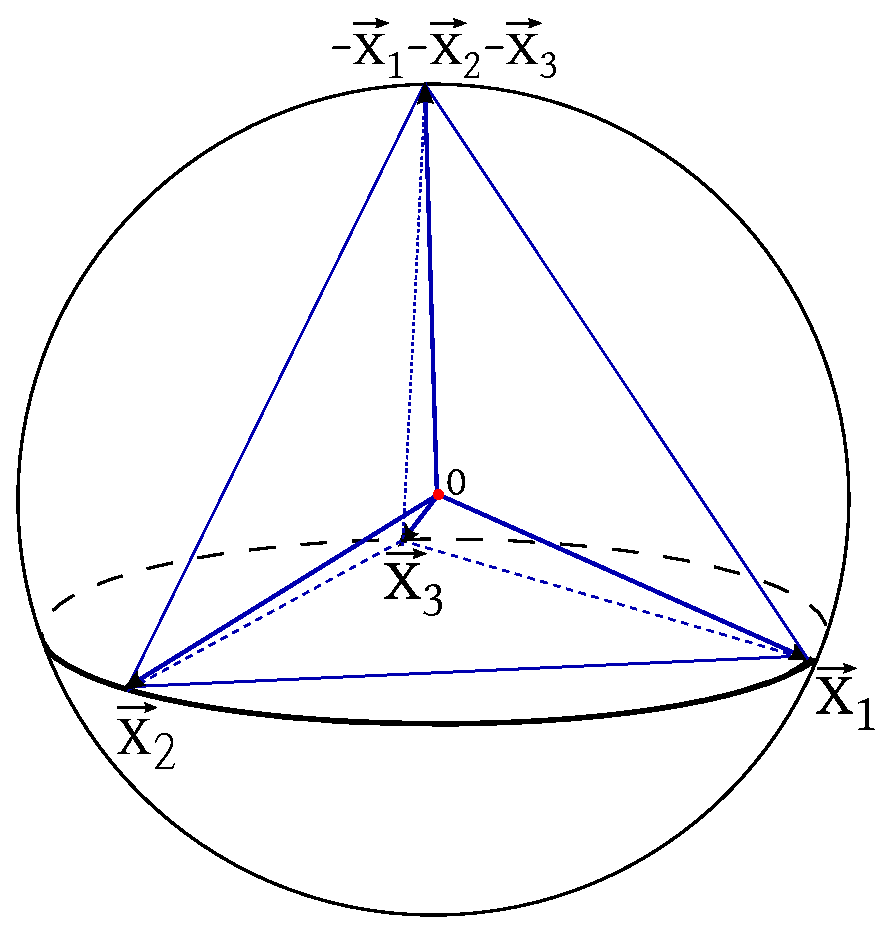
\includegraphics[scale=0.38]{tetrahedron}
	\caption[Balanced Configuration]{A regular tetrahedron ($3-$simplex) represents a balanced configuration for $k=3$.}
	\label{fig:Tetrahedron}
\end{figure}

\begin{corollary} \label{cor:NumberOfSolutions}
	Let $k,t$ be fixed. Then the expected number of solutions to the Configuration problem with input lists of size $|L|$ is
	\begin{equation} \label{eq:ExpNumberOfSolutions}
	\E[\# \text{solutions}] = \softO \left( |L|^k \Bigl(\frac{t^2}{k} \Bigl( \frac{k^2-t^2}{k^2-k} \Bigr)^{k-1}  \Bigr)^{\tfrac{n}{2}} \right).
	\end{equation}
\end{corollary}
\begin{proof}
	The total number of $k$-tuples is $|L|^k$. From Thms.~\ref{thm:WishartDist} and \ref{thm:maxConfig}, the probability that a random $k$-tuple forms a configuration from $\ConfSpacet$ is $\softO( \det(\Cbalt)^{n/2})$. Thm.~\ref{thm:maxConfig} states the value for this determinant.
\end{proof}

As a consequence, we can easily compute the size of input lists for a desired output list's size. In algorithms for \SVP, $t=1$ and the output list is required to have the same size as input lists. The following corollary proves the conjecture stated in \cite{BLS16}.

\begin{corollary} \label{cor:BalancedListSizes}
Let $k$ be fixed and $t=1$. In the Configuration problem, for the input lists each of size $|L|$, the output list is expected to be of size $|L|$ if $|L|  = \softO \Bigl( \Bigl( \frac{k^{\tfrac{k}{k-1}}}{k+1} \Bigr)^{\tfrac{n}{2}} \Bigr)$. 
\end{corollary}
\begin{proof}
	The statement immediately follows from setting the expression in Eq.~(\ref{eq:ExpNumberOfSolutions}) equal to $|L|$ for $t=1$. 
\end{proof}

Finally, we argue that solving the Configuration Problem gives a $1-\smallo(1)$ fraction of solutions for the $k$-List problem. This follows from Thm.~\ref{thm:maxConfig}. Essentially it states that for any fixed $\eps>0$, the probability that a randomly chosen solution to the approximate $k$-List problem forms a configuration $\eps$-close to $\Cbalt$, converges exponentially to $1$ as $n \rightarrow \infty$. Therefore, solving the $k$-List Configuration problem for $\CbalOne$ and restricting to only those solutions whose sum is at most $t$, gives a $1-\smallo(1)$ fraction of solutions for the approximate $k$-List problem. These arguments justify the following corollary.

\begin{corollary}\label{cor:ReductionToConfigProblem}
Let $k,t$ be fixed. Then the approximate $k$-List problem with target length $t$ can be solved in the same time as the $k$-List configuration problem with target configuration $\Cbalt$ for any fixed $\eps>0$.
\end{corollary}

\subsection{Algorithm} \label{subsec:KListAlgL2}

\begin{algorithm}[H]
\caption{$k$-List for the Configuration Problem}
\label{alg:AlgConfig}
\textbf{Input:} $L_1, \ldots, L_k$ -- lists of vectors from $\Sphere{n}$. $\Conf_{i,j}=\ScProd{\xvec_i}{\xvec_j} \in \R^{k \times k}$ -- Gram matrix. $\eps>0$. \\
\textbf{Output:} $\Lout$ -- list of $k$-tuples $\xvec_1 \in L_1, \ldots, \xvec_k \in L_k$, s.t.\ $\abs{\ScProd{\xvec_i}{\xvec_j}-\Conf_{ij}} \leq \eps$, for all $i,j$.

\begin{algorithmic}[1]

\State $\Lout \gets \{ \}$ 
\ForAll { $\xvec_1 \in L_1$}
	\ForAll {$j=2 \ldots k$}
		\State $L_j^{(1)} \gets$ \Call{Filter}{$\xvec_1, L_j, \Conf_{1,j}, \eps$} 
	\EndFor
	
	\ForAll {$\xvec_2 \in L_2^{(1)}$}
		\ForAll {$j=3 \ldots k$}
			\State $L_j^{(2)} \gets$ \Call{Filter}{$\xvec_2, L_j^{(1)}, \Conf_{2,j}, \eps$} 
		\EndFor	
		\State $\ddots$
		\Indent
			\ForAll {$\xvec_k \in L_k^{(k-1)}$}
				\State $\Lout \gets \Lout  \union \{(\xvec_1, \ldots \xvec_k)\}$
			\EndFor
		\EndIndent
	\EndFor
\EndFor 

\State{} \Return{$\Lout$} 
\end{algorithmic}
\vspace{10pt}
\begin{algorithmic}[1]
	\Function{Filter}{$\xvec, L, c, \eps$}
		\State $L' \gets \{ \}$
		\ForAll {$\xvec' \in L$}	
			\If{$\abs{\ScProd{\xvec}{\xvec'} - c}  \leq \eps$}
			 	\State $L' \gets L' \cup \{ \xvec' \}$
			\EndIf	
		\EndFor
		\State{} \Return $L'$
	\EndFunction
\end{algorithmic}

\end{algorithm}

Now we are ready to describe our algorithm for the Configuration problem given in Def.~\ref{def:ConfigProblem}.

On input the algorithm receives $k$ lists $L_1, \ldots, L_k$, a target configuration $\Conf$ in the form of a Gram matrix $\Conf_{i,j}=\langle{\xvec_i,}{\xvec_j}\rangle \in \R^{k \times k}$ and a small $\eps>0$.
The algorithm proceeds as follows: it picks an $\xvec_1 \in L_1$ and filters all the remaining lists with respect to the values $\ScProd{\xvec_1}{\xvec_i}$ for all $2 \leq i \leq k$.
More precisely, $\xvec_i \in L_i$ `survives' the filter if $\abs{\ScProd{\xvec_1}{\xvec_i} - \Conf_{1,i}}  \leq \eps$.
We put such an $\xvec_i$ into $L_i^{(1)}$ (the superscript indicates how many filters were applied to the original list $L_i$).
On this step, all the $k$-tuples of the form $(\xvec_1, \xvec_2, \ldots, \xvec_k) \in \{\xvec_1\} \times L_2^{(1)} \times \ldots \times L_k^{(1)}$ with the first vector $\xvec_1$ fixed partially match the target configuration. 
Most importantly, the lists $L_i^{(1)}$ become much shorter than the original ones. 

Next, we take $\xvec_2 \in L_2^{(1)}$ and create smaller lists $L_i^{(2)}$ from $L_i^{(1)}$ by filtering out all the $\xvec_i \in L_i^{(1)}$ that do not satisfy $\abs{\ScProd{\xvec_2}{\xvec_i} - \Conf_{2,i}}  \leq \eps$ for all $3 \leq i \leq k$.
A tuple of the form $(\xvec_1, \xvec_2, \xvec_3, \ldots, \xvec_k) \in \{\xvec_1\} \times \{\xvec_2\} \times L_3^{(2)} \times \ldots \times  L_k^{(2)}$ satisfies the target configuration $\Conf_{i,j}$ for $i=1,2$. Now we have the first two vectors fixed. 

We proceed with this list-filtering strategy until we have all $\xvec_i$ for $1\le i \le k$ fixed.
We output all the survived $k$-tuples.
Note that our algorithm becomes the trivial brute-force search algorithm once we are down to 2 lists $L_{k-1}^{(k-2)}, L_k^{(k-2)}$.
As soon as we have fixed $\xvec_1,\ldots,\xvec_{k-2}$ and created $L_{k-1}^{(k-2)},L_{k}^{(k-2)}$, we iterate over $L_{k-1}^{(k-2)}$ and check scalar products with every element from $L_{k}^{(k-2)}$. Our algorithm is detailed in Alg.~\ref{alg:AlgConfig}.

In Fig.~\ref{fig:AlgDescription}, we stress the difference between our algorithm (left) and the algorithm for the Configuration problem presented in \cite{BLS16} (right). While not being stated in terms of configurations, the BLS algorithm actually does search for tuples that form the balanced configuration but differently: for a fixed $\xvec_1$, it only filters the next list $L_2$ and the remaining $L_3, \ldots, L_k$ are left unchanged. Once $\xvec_2 \in L_2^{(1)}$ is chosen next, $L_3^{(2)}$ is obtained by applying filtering to the input $L_3$, while our Alg.~\ref{alg:AlgConfig} filters a smaller $L_3^{(1)}$. Certainly, in our approach we can miss some solutions that would be found by the BLS algorithm, but the results of Sect.~\ref{subsec:ConfigL2} show that this is a tiny fraction of solutions which vanishes in the asymptotics. To see the effect of this fact in practice, we refer the reader to Sect.~\ref{subsec:KListResults}.
\clearpage

\begin{figure}
\centering
\begin{subfigure}[t]{0.45\textwidth}
	\begin{tikzpicture}
	\tikzset{
    List/.style={
    rectangle, 
    rounded corners, 
    draw=black, thick,
    minimum width=0.9cm, 
    text centered},
    Vertex/.style={
  	ellipse,
  	draw=black, thick,
  	inner sep=1pt},
	}
	\matrix (m) [row sep=2mm, column sep=2.3mm, name=m] {
		\node[List, minimum height=50pt] (L1) {$L_1$}; &
	 	\node[List, minimum height=50pt] (L2) {$L_2$}; &
		\node[List, minimum height=50pt] (L3) {$L_3$}; &	 	
	 	\node[] {$\ldots$}; &
	 	\node[List, minimum height=50pt] (Lk) {$L_k$}; \\
	 	
	 	\node[Vertex, label=below:{\footnotesize $\xvec_1$}] (x1) {}; &
	 	\node[Vertex] (l12) {\tiny Filter}; &
	 	\node[Vertex] (l13) {\tiny Filter}; &
	 	\node[] (dots1) {}; &
	 	\node[Vertex] (l1k) {\tiny Filter}; \\
	 	
	 	\node[] {}; &
	 	\node[List, minimum height=35pt] (L2p) {$L_2^{(1)}$}; &
		\node[List, minimum height=35pt] (L3p) {$L_3^{(1)}$}; &	 	
	 	\node[] {$\ldots$}; &
	 	\node[List, minimum height=35pt] (Lkp) {$L_k^{(1)}$}; \\
	 	
	 	\node[] {}; &
	 	\node[Vertex, label=below:{\footnotesize $\xvec_2$}] (x2) {}; &
	 	\node[Vertex] (l23) {\tiny Filter}; &
	 	\node[] (dots2) {}; &
	 	\node[Vertex] (l2k) {\tiny Filter}; \\
	 	
	 	\node[] {}; &
	 	\node[] {}; &
	 	\node[List, minimum height=20pt] (L3pp) {$L_3^{(2)}$}; &
	 	\node[] {}; &
	 	\node[List, minimum height=20pt] (Lkpp) {$L_k^{(2)}$}; \\
	 	
	 	\node[] {}; &
	 	\node[] {}; &
	 	\node[] {}; &
	 	\node[] {}; &
	 	\node[] {$\vdots$};\\
	 	
	 	\node[] {}; &
	 	\node[] {}; &
	 	\node[] {}; &
	 	\node[List, minimum height=17pt] (Llast1) {\small $L_{\scalebox{0.5}{ $k-1$}}^{\scriptscriptstyle(k-2)}$}; &
	 	\node[List, minimum height=17pt] (Llast2) {\small $L_{\scalebox{0.5}{$k$}}^{\scriptscriptstyle(k-2)}$};\\
	 	
	 	\node[minimum height=10pt] {}; &
	 	\node[] {}; &
	 	\node[] {}; &
	 	\node[] {}; &
	 	\node[] {}; & \\
	 	
	 	\node[minimum height=10pt] {}; &
	 	\node[] {}; &
	 	\node[] {}; &
	 	\multicolumn{2}{r}{\node[List, minimum height=17pt] (Lout) {\small $\Lout$};} \\
	 };
	%\node[fit=(m-9-3)(m-9-5)] (Lout) {\small $\Lout$};
	 \draw (L1) -- (x1);
	 \draw[->] (x1) -- (l12);
	 \draw[->] (L2) -- (l12);
	 \draw[->] (l12) -- (L2p);
	 
	 \draw (l12) -- (l13);
	 \draw[->](L3) -- (l13);
	 \draw[->] (l13) -- (L3p);
	 
	 \draw[->] (dots1) -- (l1k);
	 \draw[->] (Lk) -- (l1k);
	 \draw[->] (l1k) -- (Lkp);
	 
	 \draw (L2p) -- (x2);
	 \draw[->] (x2) -- (l23);
	 \draw[->] (L3p) -- (l23);
	 \draw[->] (l23) -- (L3pp);
	 
	 \draw[->] (dots2) -- (l2k);
	 \draw[->] (Lkp) -- (l2k);
	 \draw[->] (l2k) -- (Lkpp);
	 
	 \draw[->] (Llast1) -- (44pt, -112pt);
	 \draw[->] (Llast2) -- (45pt, -112pt);	
	 
\end{tikzpicture}
\caption{\footnotesize Pictorial representation of Alg.~\ref{alg:AlgConfig}. At level $i$, a filter receives as input $\xvec_i \in L_i^{(i-1)}$ and a vector $\xvec_{j}$ from $L_{j}^{(i-1)}$ (for the input lists, $L = L^{(0)}$). $\xvec_j$ passes through the filter if $\abs{\ScProd{\xvec_i}{\xvec_j} - \Conf_{i,j}}  \leq \eps$, in which case it is added to $L_{j}^{(i)}$. All the vectors from $L_j^{(i-1)}$ for all $j \leq i+1$ are processed in this manner. The configuration $\Conf$ and $\eps>0$ are global parameters.}
\label{fig:AlgDescription}
\end{subfigure} %
\quad \quad
\begin{subfigure}[t]{0.47\textwidth}
	\begin{tikzpicture}
	\tikzset{
    List/.style={
    rectangle, 
    rounded corners, 
    draw=black, thick,
    minimum width=0.9cm, 
    text centered},
    Vertex/.style={
  	ellipse,
  	draw=black, thick,
  	inner sep=1pt},
	}
	\matrix (m) [row sep=1.6mm, column sep=2.3mm] {
		\node[List, minimum height=50pt] (L1) {$L_1$}; &
	 	\node[List, minimum height=50pt] (L2) {$L_2$}; &
		\node[List, minimum height=50pt] (L3) {$L_3$}; &	 	
	 	\node[] {$\ldots$}; &
	 	\node[List, minimum height=50pt] (Lk) {$L_k$}; \\
	 	
	 	\node[Vertex, label=below:{\footnotesize $\xvec_1$}] (x1) {}; &
	 	\node[Vertex] (l12) {\tiny Filter}; &
	 	\node[] (l13) {}; &
	 	\node[] (dots1) {}; &
	 	\node[] (l1k) {}; \\
	 	
	 	\node[] {}; &
	 	\node[List, minimum height=35pt] (L2p) {$L_2^{(1)}$}; &
		\node[] (L3p) {}; &	 	
	 	\node[] {$\ldots$}; &
	 	\node[] (Lkp) {}; \\
	 	
	 	\node[] {}; &
	 	\node[Vertex, label=below:{\footnotesize $\xvec_2$}] (x2) {}; &
	 	\node[Vertex] (l23) {\tiny Filter}; &
	 	\node[] (dots2) {}; &
	 	\node[] (l2k) {$\vdots$}; \\
	 	
	 	\node[] {}; &
	 	\node[] {}; &
	 	\node[List, minimum height=20pt] (L3pp) {$L_3^{(2)}$}; &
	 	\node[] {$\vdots$}; &
	 	\node[] (Lkpp) {}; \\
	 	
	 	\node[] {}; &
	 	\node[] {}; &
	 	\node[] {}; &
	 	\node[] {}; &
	 	\node[] {}; & \\[-1.3ex]
	 	
	 	\node[] {}; &
	 	\node[] {}; &
	 	\node[] {}; &
	 	\node[List, minimum height=17pt] (Llast1) {\small $L_{\scalebox{0.5}{ $k-1$}}^{\scriptscriptstyle(k-2)}$}; &
	 	\node[] {};\\
	 	
	 	\node[] {}; &
	 	\node[] {}; &
	 	\node[] {}; &
	 	\node[] {}; &
	 	\node[List, minimum height=17pt] (Llast2) {\small $L_{\scalebox{0.5}{ $k$}}^{\scriptscriptstyle(k-2)}$}; \\
	 	
	 	\node[minimum height=10pt] {}; &
	 	\node[] {}; &
	 	\node[] {}; &
	 	\node[] {}; &
	 	\node[] {}; & \\
	 	
	 	\node[minimum height=10pt] {}; &
	 	\node[] {}; &
	 	\node[] {}; &
	 	\multicolumn{2}{r}{\node[List, minimum height=17pt] (Lout) {\small $\Lout$};} \\
	 };
	 \draw (L1) -- (x1);
	 \draw[->] (x1) -- (l12);
	 \draw[->] (L2) -- (l12);
	 \draw[->] (l12) -- (L2p);
	 
	 %\draw (l12) -- (l13);
	 \draw[->](L3) -- (l23);
	 \draw[->] (l23) -- (L3pp);
	 
	 %\draw[->] (dots1) -- (l1k);
	 %\draw[->] (Lk) -- (l1k);
	 %\draw[->] (l1k) -- (Lkp);
	 
	 \draw (L2p) -- (x2);
	 \draw[->] (x2) -- (l23);
	 %\draw[->] (L3p) -- (l23);
	 %\draw[->] (l23) -- (L3pp);
	 
	 %\draw[->] (dots2) -- (l2k);
	 \draw[-] (Lk) -- (l2k);
	 \draw[->] (l2k) -- (Llast2);
	 \draw[->] (Llast1) -- (44pt, -112pt);
	 \draw[->] (Llast2) -- (45pt, -112pt);	
\end{tikzpicture}
\caption{\footnotesize The $k$-List algorithm given in \cite{BLS16}. The main difference is that a filter receives as inputs $\xvec_i$ and a vector $\xvec_j \in L_j$, as opposed to $\xvec_j \in L_j^{(i-1)}$. Technically, in \cite{BLS16}, $\xvec_i$ survives the filter if $\normalabs{\ScProd{\xvec_i}{\xvec_1+\ldots+\xvec_{i-1}}} \geq c_i$ for some predefined $c_i$. Due to our concentration results, this description is equivalent to the one given in \cite{BLS16} in the sense that the returned solutions are (up to a sub-exponential fraction) the same.}
\label{fig:AlgBLS}
\end{subfigure}
\caption[$k$-List algorithms for the Configuration problem]{$k$-List Algorithms for the Configuration Problem (Def.~\ref{def:ConfigProblem}). Left: Our Alg.~\ref{alg:AlgConfig}. Right: The algorithm from \cite{BLS16}}
\end{figure}

\clearpage

\subsection{Analysis} \label{subsec:KListAnalysisL2}

In this section we analyze the complexity of Alg.~\ref{alg:AlgConfig} for the Configuration problem. First, we should mention that the memory complexity is completely determined by the input list-sizes $\abs{L_i}$ (remember that we restrict to constant $k$) and the application of $k$ filters does not change the asymtotics. In practice, all intermediate lists $L_i^{(j)}$ can be implemented by storing pointers to the elements of the original lists. 

In the following, we compute the expected sizes of filtered lists $L_i^{(j)}$ and establish the expected running time of Alg.~\ref{alg:AlgConfig}. Since our algorithm has an exponential running time $2^{cn}$ for some $c = \Theta(1)$, we are interested in determining $c$. We ignore polynomial factors, e.g.\ we do not take into account time spent for computing inner products. 

\begin{thm}\label{thm:RunTimeAlg1}
Let $k$ be fixed. Alg.~\ref{alg:AlgConfig} given as input $k$ lists $L_1, \ldots, L_k \subset \Sphere{n}$ of the same size $\abs{L}$, a target balanced configuration $\Cbalt \in \R^{k \times k}$, a target length $0 < t < \sqrt{k}$, and $\eps > 0$, outputs the list $\Lout$ of solutions to the Configuration problem. The expected running time of Alg.~\ref{alg:AlgConfig} is
	\begin{equation}\label{eq:RunTime}
	 T =  \softO \Bigl( \abs{L} \cdot \max\limits_{1 \leq i \leq k-1}  \abs{L}^i \cdot \frac{(k^2-t^2)^i}{(k^2-k)^{i+1}}  \cdot \Bigl( \frac{(k^2 - k + (i-1)(t^2-k))^2}{k^2 - k +(i-2)(t^2-k)} \Bigr)^{\frac{n}{2}} \Bigr).
  \end{equation}
In particular, for $t=1$ and $\abs{\Lout} = \abs{L}$ it holds that
  \begin{equation}\label{eq:RunTime=1}
	 T = \softO \biggl( \Bigl( \frac{k^{ \frac{1}{k-1} }}{k+1} \cdot  \max\limits_{1 \leq i \leq k-1} k^{\frac{i}{k-1}} \cdot \frac{(k-i+1)^2}{k-i+2}  \Bigr)^{\frac{n}{2}} \biggr).
  \end{equation}
\end{thm}

\begin{remark}\label{rmk:RunningTimeOfBLS} In the proof below we also show that the expected running time of 
the BLS
$k$-List algorithm 
from \cite{BLS16} for $t=1,\abs{\Lout}=\abs{L}$ is
\begin{equation} \label{eq:RunTimeBLS}
	T_{\text{BLS}} = \softO \Bigl(  \Bigl( \frac{k^{\frac{k}{k-1}}}{(k+1)^2} \cdot \max\limits_{1 \leq i \leq k-1} \bigl( k^{\frac{i}{k-1}} \cdot (k-i+1) \bigr)\Bigr)^{\frac{n}{2}} \Bigr).
\end{equation}
\end{remark} 

\begin{proof}[Proof of Thm.~\ref{thm:RunTimeAlg1}]
	The correctness of the algorithm is straightforward: let us associate the lists $L^{(i)}$ with a level $i$, where $i$ indicates the number of filtering steps applied to $L$ (we identify the input lists with the $0\th$ level: $L_i=L^{(0)}_i$). So for executing the filtering for the $i\th$ time, we choose an $\xvec_{i} \in L_{i}^{(i-1)}$ that satisfies the condition $\abs{\ScProd{\xvec_i}{\xvec_{i-1}} - C_{i,i-1}} \leq \eps$ (for a fixed $\xvec_{i-1}$) and append to a previously obtained $(i-1)$-tuple $(\xvec_1, \ldots, \xvec_{i-1})$. Thus, on the last level, we put into $\Lout$ a $k$-tuple $(\xvec_1, \ldots, \xvec_{k})$ that is a solution to the Configuration problem. To make the subscripts less confusing, we set $C = \Cbalt$ throughout the proof. 
	
	Let us first estimate the size of the list $L_i^{(i-1)}$ output by the filtering process applied to the list $L_i^{(i-2)}$ for $i>1$ (i.e.\ the left-most lists in Fig.~\ref{fig:AlgDescription}). Recall that all $\xvec_i \in L_i^{(i-1)}$ satisfy $\abs{\ScProd{\xvec_i}{\xvec_{j}} - C_{i,j}} \leq \eps$, $1 \leq j \leq i-1 $. Then the \emph{total} number of $i$-tuples $(\xvec_1, \xvec_2, \ldots, \xvec_i) \in L_1 \times L_2^{(1)} \times \ldots \times L_i^{(i-1)}$ considered by the algorithm is determined by the probability that in a random $i$-tuple, all pairs $(\xvec_j, \xvec_{j'}), 1 \leq j,j' \leq i$ satisfy the inner product constraints given by $C_{j,{j'}}$. This probability is given in Thm.~\ref{thm:WishartDist} and, since the input lists are of the same size $\abs{L}$, we have\footnote{Throughout this proof, the equations that involve list-sizes $\abs{L}$ and running time $T$ are assumed to have $\softO(\cdot)$ on the right-hand side. We omit it for clarity.}
	\begin{align}\label{eq:ProductOfListSizes}
			\normalabs{L_1} \cdot \normalabs{L_2^{(1)}} \cdot \ldots \normalabs{L_i^{(i-1)}} = \normalabs{L}^i \cdot  \det (C[1 \ldots i])^{\frac{n}{2}},
	\end{align}	
where $\det(C[1 \ldots i])$ denotes the $i$-th principal minor of $C$.
Using Eq.~\eqref{eq:ProductOfListSizes} for two consecutive values of $i$ and dividing one equation by the other, we obtain
	\begin{align}\label{eq:IntermSize}
		\normalabs{L_{i+1}^{(i)}} = \abs{L} \cdot \Bigl( \frac{\det (C[1 \ldots i+1]}{\det (C[1 \ldots i])} \Bigr)^{\frac{n}{2}}.
	\end{align}
Note that these expected list sizes can be smaller than 1. This should be thought of as the inverse probability that the list is not empty.
Since our target is a balanced configuration $\Cbalt$, the entries of the input Gram matrix are specified by Thm.~\ref{thm:maxConfig} and, hence, we compute the determinants in the above quotient by applying Lemma~\ref{lem:CBalancedDet} with $a = \frac{t^k-k}{k^2-k}$. Again, from the shape of the Gram matrix $\Cbalt$ and the equally-sized input lists, it follows that the filtered list on each level are of the same size: $\normalabs{L_{i+1}^{(i)}} = \normalabs{L_{i+2}^{(i)}} = \ldots = \normalabs{L_k^{(i)}}$. Therefore, for all filtering levels $0 \leq j \leq k-1$ and for all $j+1 \leq i \leq k$,
  \begin{equation}\label{eq:IntermSizeExpanded}
	 \bigabs{L_i^{(j)}} = \abs{L} \cdot \Bigl( \frac{k^2 - t^2}{k^2 - k} \cdot \frac{k^2 - k + j(t^2-k)}{k^2 - k +(j-1)(t^2-k)} \Bigr)^{ \frac{n}{2} }.
  \end{equation}
Now let us discuss the complexity of the algorithm. Clearly, the running time of Alg.~\ref{alg:AlgConfig} is (up to sub-exponential factors in $n$) 
\begin{align*}
   T = \normalabs{L_1^{(0)}} \cdot (\normalabs{L_2^{(0)}} + \normalabs{L_2^{(1)}} \cdot (\normalabs{L_3^{(1)}} +\normalabs{L_3^{(2)}} \cdot(\ldots \cdot (\normalabs{L_k^{(k-2)}} + \normalabs{L_k^{(k-1)}} ) )).
\end{align*}  
Multiplying out and observing that $\normalabs{L_k^{(k-2)}}>\normalabs{L_k^{(k-1)}}$ (so creating a filtered list takes longer than enumerating over it), we may ignore the very last term and deduce that the total running time is (up to sub-exponential factors) given by

  \begin{equation} \label{eq:RunTimeProof}
  	T =  \abs{L} \cdot \max\limits_{1 \leq i \leq k-1}  \normalabs{L^{(i-1)}} \cdot \prod_{j=1}^{i-1} \normalabs{L^{(j)}},
  \end{equation}
  where $\normalabs{L^{(j)}}$ is the size of any filtered list on level $j$ (so we omit the subscripts). Consider the value $\im$ of $i$, where the maximum is attained in the above formula. The meaning of $\im$ is that the total cost over all loops to create the lists $L_j^{(\im)}$ dominates the running time. At this level, the lists $L_j^{(\im)}$ become small enough such that iterating over them (i.e.\ creating $L_j^{(\im+1)}$) does not contribute to the asymptotics. Plugging in Eqns.~\eqref{eq:ProductOfListSizes} and \eqref{eq:IntermSize} into Eq.~\eqref{eq:RunTimeProof}, we obtain
  \vspace{-1ex}
  \begin{equation}\label{eq:TotalRunningTimeViaDets}
    T=\abs{L}\cdot \max\limits_{1\le i \leq k-1} \normalabs{L}^i \Bigl( \frac{(\det C[1\ldots i])^2}{\det C[1\ldots (i-1)]}\Bigr)^{\frac{n}{2}}.
  \end{equation}
  From Lemma~\ref{lem:CBalancedDet}, $\det C[1\ldots i] = \Bigl( 1 + (i-1)\frac{t^2-k}{k^2-k})\Bigr) \Bigl( \frac{k^2-t^2}{k^2-k} \Bigr)^{i-1}$, giving us the desired expression for the running time.
  
  For the case $t=1$ and $\normalabs{\Lout} = \normalabs{L}$, the result of Cor.~\ref{cor:BalancedListSizes} on the size of the input lists $\abs{L}$ yields a compact formula for the filtered lists:
    \vspace{-1ex}
    \begin{equation}\label{eq:IntermSize_t=1}
    	\bigabs{L_i^{(j)}} =  \Bigl( k^{\frac{1}{k-1}} \cdot \frac{k-j}{k-j+1} \Bigr)^{\tfrac{n}{2}}.
    \end{equation}
    Plugging this into either Eq.~\eqref{eq:RunTimeProof} or Eq.~\eqref{eq:TotalRunningTimeViaDets}, the running time stated in Eq.~\eqref{eq:RunTime=1} easily follows.
    
    It remains to show the complexity of the BLS algorithm \cite{BLS16}, claimed in Rmk.~\ref{rmk:RunningTimeOfBLS}. The algorithm is illustrated in Fig.~\ref{fig:AlgBLS}. We change the presentation of the algorithm to our configuration setting: in the original description, a vector $\xvec_i$ survives the filter if it satisfies $\abs{ \ScProd{\xvec_i}{\xvec_1 + \ldots + \xvec_{i-1}}} \geq c_i$ for a predefined $c_i$ (a sequence $(c_1, \ldots, c_{k-1}) \in \R^{k-1}$ is given as input to the BLS algorithm). Our concentration result (Thm.~\ref{thm:WishartDist}) also applies here and the condition $\abs{ \ScProd{\xvec_i}{\xvec_1 + \ldots + \xvec_{i-1}}} \geq c_i$ is equivalent to a pairwise constraint on the scalar product $\ScProd{\xvec_i}{\xvec_j}$ up to losing an exponentially small fraction of solutions. The optimal sequence of $c_i$'s corresponds to the configuration $\Cbalt$ derived in Thm.~\ref{thm:maxConfig}.
    
    Indeed, Table 1 in \cite{BLS16} matches $\Cbalt$ (case $t=1$) exactly. So we may rephrase their filtering where instead of shrinking the list $L_i$ by taking inner products with the sum $\xvec_1+ \ldots + \xvec_{i-1}$, we filter $L_i$ by considering $\ScProd{\xvec_i}{\xvec_j}$ for $1 \leq j \leq i-1$. 
      
    It follows that the filtered lists $L^{(i)}$ on level $i$ are of the same size (in leading order) for both our and BLS algorithms.
    In particular, Eq.~\eqref{eq:IntermSize} holds for the expected list-sizes of the BLS algorithm.
    
    The crucial difference lies in the construction of these lists. To construct the list $L_i^{(i-1)}$ in BLS, the filtering procedure is applied not to $L_i^{(i-2)}$ but to a (larger) input-list $L_i$. Hence, the running time of the BLS algorithm ignoring sub-exponential factors, is (cf.\ Eq.~\eqref{eq:RunTimeProof})
      \begin{align*}
      	 T_{BLS} = 
      	 \normalabs{L_1} \cdot (\normalabs{L_2} + \normalabs{L_2^{(1)}} \cdot ( \normalabs{L_3} +\normalabs{L_3^{(2)}}  \cdot(\ldots \cdot (\normalabs{L_k} + \normalabs{L_k^{(k-1)}} ) ))
    	 =
      	 \normalabs{L}^2 \cdot \max\limits_{1 \leq i \leq k-1} \cdot \prod_{j=1}^{i-1} \normalabs{L^{(j)}}.
      \end{align*}
    The result follows after substituting Eq.~\eqref{eq:IntermSize_t=1} into the above product. 
\end{proof}

Both runtime expressions, Eq.~\eqref{eq:RunTime} for Alg.~\ref{alg:AlgConfig} and Eq.~\eqref{eq:RunTimeBLS} for the BLS algorithm, can be easily evaluated given $k$ and $\normalabs{L}$, see Fig.~\ref{fig:RunTimes}. The input list-sizes $\normalabs{L}$ are chosen to guarantee $\normalabs{\Lout} = \normalabs{L}$ on expectation.

\begin{SCfigure}[1.2]
	\centering
	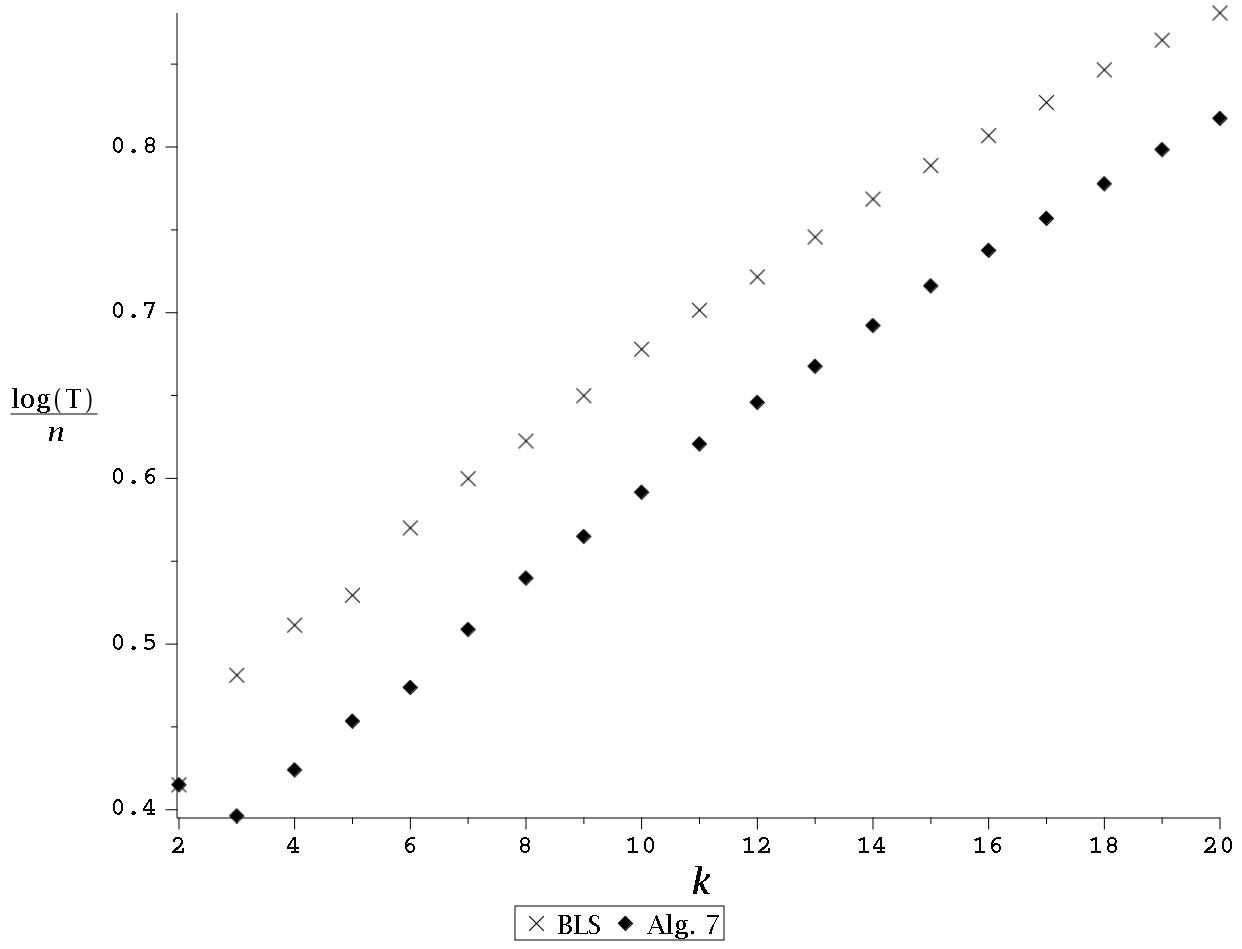
\includegraphics[scale=0.2]{kListRunTimesCompare}
	\hspace{4ex}
	\caption[Runtime exponents for $k$-List algorithms]{Running time exponents scaled by $1/n$ for the target length $t=1$. For $k=2$, both algorithms are the Nguyen-Vidick sieve \cite{NguVid08} with $\log(T)/n = 0.415$ (naive brute-force over two lists). For $k=3$, Algorithm \ref{alg:AlgConfig} achieves $\log(T)/n = 0.3962$, the BLS algorithm has $\log(T)/n = 0.4812$. \vspace{10ex}} \label{fig:RunTimes}
\end{SCfigure}

Our algorithm can be further improved by applying Locality-Sensitive Hashing techniques similar to \cite{SODA:BDGL16} to shorten the lists prior to filtering. Unfortunately, the gain is very modest: for $k=3, t=1$, we can get the running time down from $2^{0.3962n + \smallo(n)}$ to $2^{0.3717n + \smallo(n)}$. The details on this extension are presented in \cite{HK}.

We remark that it seems quite challenging to analyze the $k$-List algorithms for a \emph{non-fixed} $k$. Our approach heavily relies on the fact that $k$ is a fixed constant allowing to suppress all the pre-factors in both run-times and list sizes in the $\softO_k(\cdot)$ notation. Indeed, taking a closer look at the suppressed pre-factors, we immediately notice that they depend at least \emph{exponentially} on $k$ (see, for example, the expression for $W_{n,k}$ in Thm.~\ref{thm:WishartDist}). Being able to let $k \rightarrow \infty$ would, however, greatly contribute to our understanding of complexity of \SVP as it would enable us to compare sieving techniques with enumeration. 

Further, we do not know what is an optimal choice of $\eps$ given $k$ and $\normalabs{L}$. In Sect.~\ref{subsec:KListResults}, we present our experimental results for Alg.~\ref{alg:AlgConfig}, where we just try several $\eps$'s.

\subsection{Approximate Shortest Vector Problem} \label{subsec:ApproxSVP}

In this section we expound the connection between the approximate $k$-List problem in Euclidean norm (Def.~\ref{def:kListL2}) and the approximate Shortest Vector Problem, $\appSVP$, for a constant approximation factor $\gamma$. Recall the definition of the latter problem.

On input, we are given a full-rank lattice $\mathcal{L}(B)$ described by a matrix $B \in \R^{n \times n}$ (with polynomially-sized entries) and some constant $\gamma > 1$. The task is to output a non-zero lattice vector $\xvec \in \mathcal{L}(B)$ s.t.\ $ \| \xvec \| \leq \gamma \lambda_1 (B)$. $\xvec$ is a solution to the approximate shortest vector problem. Since the solution is not unique, we are fine with any vector that satisfies the length condition.

The family of so-called sieving (or \AKS) algorithms, described in the pioneering work of Ajtai, Kumar, and Sivakumar \cite{STOC:AjtKumSiv01}, offers the best known to-date heuristic algorithm for $\appSVP$. The fact that this algorithm achieves a single-exponential running time and memory complexity was already stated in the original paper \cite{STOC:AjtKumSiv01}, but a more precise analysis of the constant in the exponent has a long history. The result of Nguyen and Vidick in \cite{NguVid08}, stating the running time of order $2^{5.9n + \smallo(n)}$,  was later improved by Pujol and Stehl\'e to $2^{2.465n + \smallo(n)}$ running time and $2^{1.42n + \smallo(n)}$ space \cite{PujSte09}. Under an assumption on the distribution of lattice-vectors under sieving, we are able to \emph{heuristically} solve $\appSVP$ in $2^{0.415n + \smallo(n)}$ time and $2^{0.208n + \smallo(n)}$ space. Finally, the currently best known running time of  $2^{0.292n + \smallo(n)}$ in \cite{SODA:BDGL16} comes from a line of works based on the techniques from Locality-Sensitive Hashing. This is to be compared with the fastest \emph{provable} $\appSVP$ solver by Aggarwal et al.\ \cite{STOC:ADRS15}. Based on the so-called discrete Gaussian sampling, this algorithm achieves $2^{n + \smallo(n)}$-time and space complexity. 

Practically, however, sieving algorithms are less attractive than Kannan's enumeration with running time of order $2^{\bigO(n \log n)}$. This fact is attributed to exponential memory requirement of sieving (and also to the advances in pruning techniques for enumeration). Recently, Bai, Laarhoven, Stehl\'e aiming at reducing memory, presented a variant of sieving algorithm with space complexity of $2^{0.1887n+\smallo(n)}$ -- an exponential improvement over the previous $2^{0.208n + \smallo(n)}$-space sieving algorithm. Yet the gain comes at cost of increased running time: $2^{0.4812n + \smallo(n)}$ as opposed to $2^{0.415n +\smallo(n)}$ (for non-LSH sieving). To understand the BLS algorithm and how our improved $k$-List solver gives a faster sieving algorithm, we briefly explain how the \AKS algorithm works. 

\paragraph{The Nguyen-Vidick sieve.} Sieving algorithms have two flavours: the Nguyen-Vidick sieve \cite{NguVid08} and the Gauss sieve \cite{STOC:MicVou10}. Both make $\poly(n)$ number of calls to the approximate $2$-List solver. The Nguyen-Vidick sieve starts by sampling lattice-vectors $\xvec \in \Lat(B) \cap \Ball(\zerovec, 2^{\bigO(n)} \cdot \lambda_1(B))$. This can be done using, for example, Klein's sampling procedure \cite{SODA:Klein00} that outputs a lattice-vector of length not greater than $2^{\bigO(n)} \cdot \lambda_1(B)$.  In the $2$-List Nguyen-Vidick sieve, we sample many such lattice-vectors, put them in a list $L$, and search for \emph{pairs} $\xvec_1 \times \xvec_2 \in L \times L$ s.t. $\| \xvec_1 \pm \xvec_2 \| \leq (1-\eps) \max\{\| \xvec_1 \|, \| \xvec_2 \|\}$ for some small $\eps>0$. The sum is put into $\Lout$. The size of $L$ is chosen in a way to guarantee $\normalabs{L} \approx \normalabs{\Lout}$. The search for pairs is repeated over the list $\Lout$ once it is large enough. 

The size of $L$ determines the space complexity of the algorithm. A natural way to shorten the size of the input list $L$ is, instead of looking for pairs, look for triples, or, more general, $k$-tuples that form a short sum. Indeed, it easily follows from Cor.~\ref{cor:BalancedListSizes} that the larger $k$ is, the fewer vectors we should sample for the starting list  $L$ in order to expect $\normalabs{\Lout} = \normalabs{L}$. 

So the Nguyen-Vidick can be generalized to the search for $k$-tuples $\xvec_1, \ldots, \xvec_k \in L \times \ldots \times L$ s.t.\ $\| \xvec_1 + \ldots + \xvec_k \| \leq (1-\eps) \max_{1 \leq i \leq k} \{\| \xvec_i\|\}$. Now the sum $\xvec_1 + \ldots + \xvec_k$ is put into $\Lout$ and the search for $k$-tuples is repeated over $\Lout$. Note that since with each new iteration we obtain vectors that are shorter by a constant factor $(1-\eps)$, starting with $2^{\bigO(n)}$ approximation to the shortest vector (a property guaranteed by Klein's sampler applied to an \LLL-reduced basis), we need only $\poly(n)$ iterations to find the desired $\xvec \in \Lat(B)$.

Naturally, we can apply our Alg.~\ref{alg:AlgConfig} to $k$ copies of the list $L$ to implement the search for short sums. We do so by making a commonly used assumption: we assume the sampled lattice-vectors we put into the list lie uniformly on a spherical shell (on a very thin shell, essentially a sphere). The heuristic here is that it does not affect the behaviour of the algorithm. Intuitively, the discreteness of a lattice should not be `visible' to the algorithm (at least not in the search for the approximate shortest vector; as soon as we see the discreteness, the vectors are already short enough). We refer to \cite{NguVid08} for a more exhaustive discussion on this heuristic. 

The advantage in using our Alg.~\ref{alg:AlgConfig} instead of the BLS $k$-List search within an \appSVP algorithm is straightforward: the search for a `good' $k$-tuple is the routine that determines the complexity of the algorithm. So any improved algorithm for the approximate $k$-List problem immediately leads to a better \appSVP algorithm. 

\paragraph{Gauss sieve.} More interestingly, our improved $k$-List algorithm for $k \geq 3$ can as well be used within the Gauss sieve, which is known to perform faster in practice than the Nguyen-Vidick sieve. Let us briefly recall the Gauss sieve algorithm.

An iteration of the original 2-Gauss sieve as described in \cite{STOC:MicVou10}, searches for pairs $(\pvec, \vvec)$ s.t.\ $\| \pvec + \vvec \| < \max \{\| \pvec \|, \| \vvec \| \}$, where $\pvec \in \mathcal{L}(B)$ is \emph{fixed}, $\vvec \in L \subset \mathcal{L}(B)$, and $\pvec \neq \vvec$. Once such a pair is found and $\| \pvec \| > \| \vvec \|$, we reduce $\pvec$ by setting $\pvec'  \leftarrow \pvec + \vvec$ and proceed with the search over $(\pvec', \vvec)$, otherwise if $\| \pvec \| < \| \vvec \|$, we delete $\vvec \in L$ and store the sum $ \pvec + \vvec$ as $\pvec$-input point for the next iteration. Once no pair is found, we add $\pvec'$ to $L$. On the next iteration, the search is repeated with another $\pvec$ which is obtained either by reducing some previously deleted $\vvec \in L$, or by sampling from $\mathcal{L}(B)$. The idea is to keep only those vectors in $L$ that \emph{cannot} form a pair with a shorter sum. Bai, Laarhoven, and Stehl\'{e}  in \cite{BLS16}, generalize it to the $k$-Gauss sieve by keeping only those vectors in $L$ that do not form a shorter $k$-sum. In the language of configuration search, we look for configurations $(\pvec, \vvec_1, \ldots, \vvec_{k-1}) \in \pvec \times L \times \ldots \times L$ where the first point is fixed, so we apply our Alg.~\ref{alg:AlgConfig} on $k-1$ (identical) lists.

Pseudo-code for $3$-Gauss sieve is given in Alg.~\ref{alg:3GaussSieve} below. We assume the approximation $\gamma \lambda_1(B)$ is given as input. The main procedure (first lines 1-11) is exactly the same as in the original algorithm of Micciancio-Voulgaris. The difference is in the main subroutine $\Call{TripleReduce}$ that implements the approximate $3$-List search with the first vector in a triple being $\pvec$. The list $L$ is always kept sorted so that at the end of the procedure the shortest vector in the list is $L[1]$.
The algorithm can be easily generalized to the larger $k$, but we decided to present $k=3$ case as the most practically relevant. The experimental results on $3$-Gauss sieve are given in the next section.

\begin{algorithm}[t]
\caption{$3$-Gauss sieve}
\label{alg:3GaussSieve}
\textbf{Input:} $B \in \R^{n \times n}$ - an \LLL-reduced lattice basis, $\gamma \lambda_1(B)$ - the desired approximation factor, $\eps>0$ \\
\textbf{Output:} $\xvec \in \Lat(B)$ s.t.\ $\| \xvec \| \leq \gamma \lambda_1 (B)$

\begin{algorithmic}[1]
	\State $L \gets \{\}$ \Comment Sorted list of triple-reduced vectors
	\State $S \gets \{\}$ \Comment Stack of vectors
	\While{($L[1] > \gamma \lambda_1(B)$)}
		\If{$S$ is not empty}
			\State $\pvec \gets S.\text{pop()}$
		\Else
			\State $\pvec \gets \text{KleinSample}(B)$ \Comment Sample a vector from $\Lat(B)$
		\EndIf
		\State $\pvec' \gets $ \Call{TripleReduce}{$\protect \pvec, L, s$}
		\If{$\pvec' \neq \zerovec$}
			\State $L \gets L \union \{ \pvec'\}$
		\EndIf
	\EndWhile
	\State \Return $L[1]$
\end{algorithmic}

\vspace{10pt}

\begin{algorithmic}[1]
	\Function{TripleReduce}{$\protect \pvec, L, S$}
		\While{($\pvec$ cannot be reduced)} \Comment Try to reduced $\pvec$ first
			\State $L' \gets $ \Call{Filter}{$ \protect \pvec, L, \eps$}
			\ForAll{$\vvec_1, \vvec_2 \in L' \times L'$}
				\If{$\| \pvec \pm \vvec_1 \pm \vvec_2 \| < \| \pvec \|$}
					\State $\pvec \gets \vvec_1 \pm \vvec_2$ \Comment the sign should satisfy the If-condition
				\EndIf
			\EndFor
		\EndWhile
		\State $L' \gets $ \Call{Filter}{$ \protect \pvec, L$} \Comment with a new reduced $\pvec$
		\ForAll{$\vvec_1, \vvec_2 \in L' \times L'$}
			\If{$\| \pvec \pm \vvec_1 \pm \vvec_2 \| < \max \{ \| \vvec_1 \|, \| \vvec_2 \| \} $}
				\State $\max \{ \| \vvec_1 \|, \| \vvec_2 \| \} \gets \pvec \pm \vvec_1 \pm \vvec_2$
			\EndIf
		\EndFor
		\State \Return $\pvec$
	\EndFunction
\end{algorithmic}

\vspace{10pt}

\begin{algorithmic}[1]
	\Function{Filter}{$\protect \pvec, L, \eps$} \Comment Filter w.r.t.\@ balanced configuration $\Cbalt$
		\State $L' \gets \{ \}$
		\ForAll{$\vvec \in L$}
			\If{$\big| \frac{\langle \vvec, \pvec \rangle}{\|\vvec \| \|\pvec \|} \big| \geq \frac{1}{3} - \eps$}
				\State $L' \gets L' \union \{ \vvec \}$
			\EndIf
		\EndFor
		\State \Return $L'$
	\EndFunction
\end{algorithmic}

\end{algorithm}

\clearpage

\subsection{Experimental results} \label{subsec:KListResults}
We implement the $3$-Gauss sieve Algorithm~\ref{alg:3GaussSieve} in collaboration with S.\ Bai \cite{Bai16}. 
The implementation is based on the program developed by Bai, Laarhoven, and Stehl\'{e} in \cite{BLS16}. 
The experiments are run on the Ruhr University C3 cluster \cite{C3}. The results are presented in Table~\ref{table:kListExperiments}.

Lattice bases are generated by the \SVP challenge generator \cite{SVPChallenge}. It produces a lattice generated by the columns of the matrix
\begin{align*} B=
\begin{psmallmatrix}
	p & x_1 & \ldots & x_{n-1} \\
	0 & 1 & \ldots &  0  \\
	\vdots & \vdots & \ddots & \vdots \\
	0 & 0 & \ldots & 1 \\
\end{psmallmatrix},
\end{align*}
where $p$ is a large prime, and $x_i< p$ for all $i$. Lattices of this type are random in the sense of Goldstein and Mayer \cite{GoldMay06}.

For all the dimensions except $n=80$, the bases are preprocessed with \BKZ reduction of block-size~$20$. For $n=80$, the block-size is $30$. For our input lattices, we do not know their minimum $\lambda_1$. The algorithm terminates when it finds many linearly dependent triples $(\pvec, \vvec_1, \vvec_2)$. It means that at some point $\Call{TripleReduce}$ starts outputting $\zerovec$. We set a counter for such an event and terminate the algorithm once this counter goes over a pre-defined threshold. The intuition behind this idea is straightforward: at some point the list $L$ will contain very short basis-vectors and the remaining list-vectors will be their linear combinations. Trying to reduced the latter will ultimately produce the zero-vector. The same termination condition was already used in \cite{BLM15}, where the authors experimentally determine a threshold of such `zero-sum' triples.

Up to $n=64$, the experiments are repeated 5 times (i.e.\ on 5 random lattices), for the dimensions less than $80$, 3 times. For the running times and the list-sizes presented in the table below, the average is taken. For $n=80$, the experiment was performed once.  

Our tests confirm a noticeable speed-up of the 3-Gauss sieve when our Configuration Search Algorithm~\ref{alg:AlgConfig} is used. Moreover, as the analysis suggests (see Fig.~\ref{fig:RunTimes}), our algorithm outperforms the naive 2-Gauss sieve while using much less memory. 

Another interesting aspect of the algorithm is the list-sizes when compared with BLS. Despite the fact that asymptotically the size of the list $|L|$ is the same for our and for the BLS algorithms, in practice our algorithm requires a longer list (cf.\ the right numbers in each column). This is due to the fact that we filter out a larger fraction of solutions. Also notice that increasing $\eps$ -- the approximation to the target configuration -- we achieve an additional speed-up. This becomes obvious once we look at the $\Call{Filter}$ procedure: allowing for a smaller inner-product throws away less vectors, which in turn results in a shorter list $L$. For the range of dimensions we consider, the optimum is attained at $\eps=0.3$.

\renewcommand{\arraystretch}{1.9}
\begin{table}[t]
	\centering
	\resizebox{\textwidth}{!}{%
	\begin{tabular}{|c|c|c|c|c|c|c|} \hline
		 & \multirow{2}{*}{$2$-sieve} & \multirow{2}{*}{BLS $3$-sieve} & \multicolumn{4}{c|}{ Alg.~\ref{alg:3GaussSieve}, $3$-sieve} \\ \cline{4-7}
		& & & $\eps = 0.0$ & $\eps = 0.015$ & $\eps = 0.3$ & $\eps = 0.4$ \\ \hline
		$n$ & $T$, $\normalabs{L}$ & $T$, $\normalabs{L}$ & $T$, $\normalabs{L}$ & $T$, $\normalabs{L}$ & $T$, $\normalabs{L}$ & $T$, $\normalabs{L}$ \\ \hline
		60 & 1.38e3, 13257 & 1.02e4, 4936& 1.32e3, 7763& 1.26e3, 7386& 1.26e3, 6751 & \textbf{1.08e3, 6296} \\ \hline
		62 & 2.88e3, 19193 & 1.62e4, 6239 & 2.8e3, 10356 & 3.1e3, 9386 & \textbf{1.8e3, 8583} & 2.2e3, 8436 \\ \hline
		64 & 8.64e3, 24178 & 5.5e4, 8369 & 5.7e3, 13573& 3.6e3, 12369 & \textbf{3.36e3, 11142}& 4.0e4, 10934\\ \hline
		66 & 1.75e4, 31707 & 9.66e4, 10853 & 1.5e4, 17810 & 1.38e4, 16039 & \textbf{9.1e3, 14822}& 1.2e4, 14428 \\ \hline
		68 & 3.95e4, 43160 & 2.3e5, 14270 & 2.34e4, 24135 & 2.0e4, 21327 & \textbf{1.68e4, 19640}& 1.86e4, 18355 \\ \hline
		70 & 6.4e4, 58083 & 6.2e5, 19484 & 6.21e4, 32168 & 3.48e5, 26954 & \textbf{3.3e4, 25307} & 3.42e4, 24420 \\ \hline
		72 & 2.67e5, 77984 & 1.2e6, 25034& 7.6e4, 40671 & 7.2e4, 37091 & \textbf{6.16e4, 34063} & 6.35e4, 34032 \\ \hline
		74 & 3.45e5, 106654 & \textemdash& 2.28e5, 54198& 2.08e5, 47951& \textbf{2.02e5, 43661}& 2.03e5, 40882\\ \hline
		76 & 4.67e5, 142397 & \textemdash& 3.58e5, 71431& 2.92e5, 64620& \textbf{2.42e5, 56587} & 2.53e5, 54848 \\ \hline
		78 & 9.3e5, 188905 & \textemdash & \textemdash & \textemdash& \textbf{4.6e5, 74610} & 4.8e5, 70494 \\ \hline
		80 & \textemdash & \textemdash &\textemdash & \textemdash& \textbf{9.47e5, 98169} & 9.9e5, 98094\\ \hline
	\end{tabular}
	}	
	\caption[Experimental results for $k$-tuple Gauss sieve]{Experimental results for $k$-tuple Gauss sieve. The running times $T$ are given in seconds, $\abs{L}$ is the maximal size of the list $L$. $\eps$ is the approximation parameter for the subroutine $\Call{Filter}$ of Alg.~\ref{alg:3GaussSieve}. The best running-time per dimension is type-set bold.}
	\label{table:kListExperiments}
\end{table}

\clearpage

%\begin{center}
%\rule[0pt]{\textwidth}{1pt}\\[7pt]
%{\LARGE {This chapter is due}}
%\rule[0pt]{\textwidth}{1pt}
%\end{center}
\section{Approximate \SVP on a $q$-ary lattice} 
\label{sec:ApproxQary}

In this section we present a combinatorial algorithm that solves the approximate shortest vector problem, $\appSVP$, on a $q$-ary lattice. As opposed to the algorithm from the previous section where the approximation factor $\gamma$ was a constant, here $\gamma$ is polynomial in the lattice-dimension, i.e.\ we look for a vector $\vvec$ from $\qLat \subset \Z_q^n$ s.t.\ $\| \vvec \| \leq \poly(n) \lambda_1(\qLat)$.

An algorithm for $\appSVP$ with a polynomial approximation factor gives a way to solve the so-called Short Integer Solution Problem (\SIS) -- the problem introduced by Ajtai in \cite{STOC:Ajtai96} that serves as the foundation for a variety of cryptographic primitives. Given a matrix $\AMat \in \Z_q^{n \times m}$ composed column-wise from uniformly chosen $\avec_i \in \Z_q^n$, \SIS asks to find a short $\vvec \in \Z_q^m$ s.t.\ $\AMat \vvec = 0 \mod q$. The length condition is specified by an input parameter $\beta$, i.e. the output $\vvec$ must satisfy $\| \vvec \| \leq \beta$, where $ \beta=\poly(n)$ and the degree of the polynomial depends on the modulus $q$. Note that we are not interested in the trivial solution $\vvec = (q, 0, \ldots, 0)$. Also notice that if we ask for $\vvec \in \ZO{n}$, \SIS becomes the vectorial Subset Sum Problem.

To see the connection between \SIS and the approximate \SVP, let us consider an $m$-dimensional $q$-ary lattice $\qLATTp(\AMat) = \{ \xvec \in \Z^m \colon \AMat \xvec = 0 \mod q \}$. A solution to $\appSVP$ on $\qLATTp(\AMat)$ is a vector $\vvec \in \qLATTp(\AMat)$ of length $\|\vvec \| \leq \gamma \lambda_1(\qLATTp(\AMat))$ and therefore, it is a solution to the \SIS problem when $\gamma$ is appropriately chosen. From Minkowski's bound we know that $\lambda_1(\qLATTp(\AMat) \leq \sqrt{m} q^{n/m}$. Hence, if we set $q=\bigO(n^{\cq})$ (as we did in Chap.~\ref{chap:LWEasBDD} for the analysis of \LWE), $\gamma  = \bigO(n^{\cg})$ for constants $\cq>1, \cg$, and take $m = \TLandau(n)$, a solution for $\appSVP$ will be a vector of length $\|\vvec \| \leq n^{\cg + \cq/2 + 1/2}$. Values of $\cg$ stem from the connection of \SIS to the worst-case lattice-problems. Since Ajtai's proof, the constant has been improved from the original $\cg=8+\smallo(1)$ \cite{STOC:Ajtai96} down to $\cg=2.5+\smallo(1)$ in \cite{Mic05} and, finally, to $\cg=1+\smallo(1)$ in \cite{FOCS:MicReg04}. In the language of \SIS, $\cg$ is known as Ajtai's connection factor.

We have a natural restriction on $\cg$ that comes from the fact that we want to avoid trivial solutions of length $q$, namely $\cg<\cq/2 - 1/2$. 

Notice that we already mentioned $\appSVP$ in Sect.~\ref{sec:OtherAttacks} when we discussed the so-called $\Dual$ attack on \LWE. The name of the attack comes from the fact that the two problems, \LWE and \SIS, are `dual' to each other. What it means is that the \LWE problem -- the decoding problem on $\Lat(\AMat\transpose)$ -- can be solved using a \SIS oracle for $\AMat$ (or, equivalently, an oracle for $\appSVP$ on $\qLATTp(\AMat)$) as we have already seen in Alg.~\ref{alg:Dual}, Chap.~\ref{chap:LWEasBDD}. The two lattices, $\Lat(\AMat\transpose)$ and $\qLATTp(\AMat)$, are dual to each other up to scaling by $q$: $\qLat(\AMat\transpose)^* = \frac{1}{q} \qLATTp(A)$, $\qLATTp(A)^* = \frac{1}{q}\qLat(\AMat\transpose)$.  
We refer the reader to \cite{Mic10} for more interesting outcomes of this duality.

In the following sections we present two combinatorial algorithms for $\appSVP$ on $\qLATTp(\AMat)$ in case $\gamma =\poly(n)$. The second algorithm has a better constant in the running time exponent. Next, we compare our algorithms with the \BKZ reduction run on $\qLATTp(\AMat)$ when the block-size $\beta$ is chosen s.t.\ the first vector of the reduced basis is a solution to $\appSVP$. We conclude that our improved algorithm outperforms \BKZ for some values of $\cq, \cg$ even when $\BKZ$ is instantiated with the best known heuristic \SVP oracle.


\subsection{An algorithm for $\appSVP$ on a $q$-ary lattice} \label{subsec:qAryAlg}

In this section, we present a combinatorial algorithm that on input $\AMat \in \Z_q^{n \times 2n}$ and $\cg < \cq/2 - 1/2$, outputs a vector $\vvec \in \qLATTp(A) \subset \Z_q^{2n}$ s.t.\ $\| \vvec \| \leq n^{\cg+\cq/2+1/2}$. Notice that we set the lattice dimension $m$ as $m=2n$. This choice simplifies the exposition and is necessary for the improved algorithm described in Sect.~\ref{subsec:qAryAlgImproved}. Case $m=\cm n$ for $\cm = \TLandau(1)$ is considered in Rmk.~\ref{rmk:Linm}.%We make such a choice of $m$ for two reasons. First, it simplifies the description of the algorithms and, second, another constant will not make our algorithm faster. 

The algorithm is actually a combinatorial \BKW-type algorithm for \LWE due to Kirchner-Fouque \cite{C:KirFou15} and Guo et al.\ \cite{C:GuoJohSta15} adapted to the $\appSVP$ problem. We now give its high-level overview.

The idea is to split the dimension of the lattice, $2n$, into $k$ blocks $d_1, \ldots, d_k$, i.e.\ $\sum_{i=1}^k d_i = 2n$. We also choose $k$  positive values $R_1, \ldots, R_k$ where $R_i < q/2$ for all $i$. The algorithm proceeds in $k$ steps. 

On Step 1, we search for pairs of lattice-vectors $(\vvec_1, \vvec_2)$ s.t.\
\[
\Big\lfloor \frac{[\vvec_1]_1^{d_1}}{R_1} \Big\rceil =  \Big\lfloor \frac{[\vvec_2]_1^{d_1}}{R_1} \Big\rceil\footnote{Recall the notation $[\xvec]_i^j = x_i\ldots x_j$ for $i \leq j$.}.
\]
In other words, we split our $q$-ary cube $[-\frac{q-1}{2}, \frac{q-1}{2}]^{d_1}$ (assume $q$ is odd, the algorithm can be easily adapted for an even $q$) into many smaller cubes $[-R_1, R_1]^{d_1}$ and search for pairs $(\vvec_1, \vvec_2)$ that on their first $d_1$ coordinates lie in the same cube. In our algorithm we set $R_1 = n^{\smallo(1)} \ll q $, and we can adjust our choice for $R_1$ s.t. the small cubes split the large cube evenly. See Fig.~\ref{fig:Bucketing} for a $2$-dimensional example. 

Once two such vectors are found, we subtract one from the other and put the result into list $L_1$. Important is that we can bound the $\ell_{\infty}$-norm of elements in $L_1$: on average, $\| [\vvec_1 - \vvec_2]_1^{\d_1}\|_{\infty} \leq \sqrt{2}R_1$. The output of Step 1 are many vectors with \emph{bounded} $\ell_{\infty}$-norm on their first $d_1$ coordinates. On Step 2, we use vectors from $L_1$ to search for pairs that lie in the same $[-R_2, R_2]^{\d_2}$ cube on their $d_1+1, \ldots, d_2$ coordinates analogously to Step 1. The output of Step 2 is a list $L_2$ with vectors bounded in $\ell_{\infty}$-norm on coordinates $1, \ldots, d_1$ and $d_1+1, \ldots, d_2$.  

Repeating this procedure for all $k$ steps, we end up with lattice-vectors for which we can bound their $\ell_{\infty}$-norm on all the $2n$ coordinates and hence, their Euclidean norm. From the upper-bound on the length of the output, we find an optimal on $k$. We defer the discussion on how to set $R_i$'s and $k$ to the next section. 

\begin{figure}[t]
	\centering
	\begin{tikzpicture}
	\draw[gray!20, ->] (-90pt,0) -- (90pt,0);
	\draw[gray!20, ->] (0,-80pt) -- (0,80pt);
	
	 \draw[thick] (-60pt, -60pt) rectangle (60pt, 60pt);
	 \draw (-60pt, 0)  node[below left] {\scriptsize $-\tfrac{q-1}{2}$};
	 \draw (60pt, 0)  node[below right] {\scriptsize $\tfrac{q-1}{2}$};
	 
	 \draw[very thin] (-20pt, -60pt) -- (-20pt, 60pt);
	 \draw[very thin] (20pt, -60pt) -- (20pt, 60pt);
	 \draw[very thin] (-60pt, -20pt) -- (60pt, -20pt);
	 \draw[very thin] (-60pt, 20pt) -- (60pt, 20pt);
	 
	 \draw [decoration={brace, mirror, raise=7pt},
	 		decorate,below=10pt, yshift=5pt](-20pt, 0) -- (20pt, 0) node [black,midway, yshift=-8pt] {\scriptsize $R$};
	 		
	 \filldraw (45pt, 45pt) circle (1pt) node[below right, xshift=-3pt, yshift=2pt] {\tiny $\vvec_1$};
	 \filldraw (32pt, 35pt) circle (1pt) node[below left, xshift=6pt, yshift=2pt] {\tiny $\vvec_2$};
	 
	 \draw [decoration={brace, raise=5pt},
	 	 		decorate,above=10pt, yshift=-3pt, xshift=2pt](32pt, 35pt) -- (45pt, 45pt) node [black,midway, rotate=37, yshift=5pt, xshift=-4pt] {\tiny $ \leq \mkern-6mu \sqrt{2}R$};
	 	 		
	%----------LABELS---------
	\node[draw=none] at (10pt, -15pt){\tiny $(0,0)$};
	\node[draw=none] at (10pt, 25pt){\tiny $(0,1)$};	
	\node[draw=none] at (10pt, -55pt){\tiny $(0,-1)$};
	
	\node[draw=none] at (50pt, 25pt){\tiny $(1,1)$};
	\node[draw=none] at (50pt, -15pt){\tiny $(1,0)$};
	\node[draw=none] at (50pt, -55pt){\tiny $(1,-1)$};
	
	\node[draw=none] at (-30pt, 25pt){\tiny $(1,-1)$};
	\node[draw=none] at (-30pt, -15pt){\tiny $(-1,0)$};
	\node[draw=none] at (-33pt, -55pt){\tiny $(-1,-1)$};
	\end{tikzpicture}
	\caption[Bucketing on a $2$-dimensional $q$-ary lattice]{Bucketing on a $2$-dimensional $q$-ary lattice. Each small cube of length $R$ gets its two-dimensional label. The vectors $\vvec_1$, $\vvec_2$ appear in the same bucket $(1, 1)$ and, hence, the $\ell_2$-norm of their difference is bounded by $\sqrt{2}R$.}
	\label{fig:Bucketing}
\end{figure}

There is one simple trick which greatly improves the running time of the algorithm. We can write our input matrix $\AMat \in \Z_q^{n \times 2n}$ as $\AMat = [\AMat_1 | \AMat_2]$ where $\AMat_i \in \Z_q^{n \times n}$. With high probability, we have that $\AMat_1$ is invertible $\bmod~q$ allowing us to write $\AMat = [\Id_n | \AMat']$ where $\AMat' = \AMat_1^{-1} \AMat_2 \bmod q$. Essentially this procedure brings a $q$-ary code generated by $\AMat$ to a systematic form. It is easy to verify that a basis for $\qLATTp(\AMat)$ is of the form (cf. with the basis $B$ for $\qLat(\AMat\transpose)$ given in Eq.~(\ref{eq:LWEBasis})):
\begin{equation}\label{eq:BasisD}
	\DMat = \begin{pmatrix}
	-\AMat' & q\Id_n \\
	\Id_{n} & 0
	\end{pmatrix}.
\end{equation}


\begin{algorithm}[t]
	\caption{$\appSVP$ on a $q$-ary lattice}
	\label{alg:ApproxSVP}
	\textbf{Input:} $D$ -- a basis for the lattice $\qLATTp(A) \subset \Z_q^{2n}$ defined as in Eq.~(\ref{eq:BasisD}), $\gamma = n^{\cg}$ -- the approximation factor, $\cg>0$ \\
	\textbf{Output:} $L_k$ -- list of vectors from $\qLATTp(A)$ with vectors of norm $\| \vvec \| \leq n^{\cg+\cq/2+1/2}$;
	
	\begin{algorithmic}[1]
		
		\State Set the sieving bounds $R_i$ as $R_1 = n^{\smallo(1)}$ and $R_i = \sqrt{2}^{i-1} R_1$ for $i \geq 2$.
		\State Set the lengths of blocks $d_i$ as in Eq.~(\ref{eq:d_i}) and the boundaries of each block $(l_{i-1}, \ldots, l_i)$ s.t.\ $l_{i}-{l_{i-1}} = d_i$ and $l_k = 1, l_0 = n$.
		
		\Repeat \Comment{Create the list $L_0$}
		\State Choose $\xvec \in \Z_q^{2n}$ s.t.\ $\| [\xvec]_{n+1}^{2n} \|_{\infty} \leq R_1$
		\State $L_0 \gets L_0 \union \{D\xvec \bmod q\} $
		\Until{$L_0$ is large enough}
		
		\State $T \gets \emptyset$ \Comment{Initialize an array $T$ indexed by buckets}
		\ForAll {$i=1 \ldots k$} \label{algline:ForLoop1}
			\ForAll { $\vvec \in L_{i-1}$} \label{algline:ForLoop2}
				\State $b \gets \Big\lfloor \frac{[\vvec]_{l_i}^{l_{i-1}}}{R_i} \Big\rceil$ \Comment Find the bucket for $\vvec\mkern2mu[l_i, \ldots, l_{i-1}]$
				\If{$T[b] = \emptyset$}
					\State $T[b] \gets \vvec$
				\Else
					\State $L_{i} \gets L_{i} \union \{T[b] - \vvec \}$
					\State $T[b] \gets \emptyset$
				\EndIf
			\EndFor
		\EndFor
		\State \Return $L_k$
	\end{algorithmic}
	
	\vspace{10pt}
	
\end{algorithm}

\begin{figure}[H]
	\centering
	\begin{tikzpicture}[]
	\tikzset{
		List/.style={
			rectangle split, rectangle split horizontal,  
			draw=black, thick,
			%text width=10em,
			inner sep=6pt,
		} 
	}    
	\matrix (m) [row sep=0.8em, column sep=3em]{
		\node[](L0) {$L_0:$}; & 
		\node[List, rectangle split parts=3, name=list, rectangle split part fill={black!60,black!60,black!10}] (list) {
			\nodepart[text width=5.4cm]{one}{}
			\nodepart[text width=0.6cm]{two}
			\nodepart[text width=6cm] {three}};
		
		\draw [decoration={brace, raise=5pt},
		decorate,below=10pt] (list.two split north) -- (list.north east) node [black,midway, yshift=20pt] {\scriptsize $n$}; 
		
		\draw [decoration={brace,raise=5pt},
		decorate,below=10pt](list.one split north) -- (list.two split north) node [black,midway, yshift=20pt] {\scriptsize $d_1$};
		
		\draw [decoration={brace, mirror, raise=5pt},
		decorate,below=10pt](list.two split south) -- (list.south east) node [black,midway, yshift=-10pt] {\scriptsize $\leq R_1$};
		
		\draw [decoration={brace, mirror, raise=5pt},
		decorate,below=10pt](list.south west) -- (list.two split south) node [black,midway, yshift=-10pt] {\scriptsize $\leq q/2$};
		\draw [decoration={brace,raise=18pt},
		decorate,below=10pt](list.north west) -- (list.north east) node [black,midway,yshift=30pt] {\scriptsize $2n$};\\[-1ex]
		%---------------------------------------  
		\node[](L1) {$L_1:$}; & 
		\node[List, rectangle split parts=4, name=list2, rectangle split part fill={black!60,black!60,black!15,black!15}] (list2) {
			\nodepart[text width=4.2cm]{one}{}
			\nodepart[text width=0.8cm]{two}
			\nodepart[text width=0.6cm] {three}
			\nodepart[text width=6cm] {four}};
		
		\draw [decoration={brace,raise=5pt},
		decorate,below=10pt](list2.three split north) -- (list2.north east) node [black,midway, yshift=20pt] {\scriptsize $n$}; 
		
		\draw [decoration={brace,raise=5pt},
		decorate,below=10pt](list2.two split north) -- (list2.three split north) node [black,midway, yshift=20pt] {\scriptsize $d_1$};
				
				
		\draw [decoration={brace, mirror, raise=5pt},
		decorate,below=10pt](list2.two split south) -- (list2.south east) node [black,midway, yshift=-10pt] {\scriptsize $\leq \sqrt{2}R_1$};

		
		\draw [decoration={brace,raise=5pt},
		decorate,below=10pt](list2.one split north) -- (list2.two split north) node [black,midway, yshift=20pt] {\scriptsize $d_2$};
		
		\draw [decoration={brace, mirror, raise=5pt},
		decorate,below=10pt](list2.south west) -- (list2.two split south) node [black,midway, yshift=-10pt] {\scriptsize $\leq q/2$};\\ [-1ex]
		
		%---------------------------------------  
		\node[](L2) {$L_2:$}; & 
		\node[List, rectangle split parts=5, name=list3, rectangle split part fill={black!60,black!60,black!30,black!30,black!30}] (list3) {
					\nodepart[text width=3.0cm]{one}{}
					\nodepart[text width=0.8cm]{two}
					\nodepart[text width=0.8cm]{three}
					\nodepart[text width=0.6cm] {four}
					\nodepart[text width=6cm] {five}};
				
		\draw [decoration={brace,raise=5pt},
		decorate,below=10pt](list3.four split north) -- (list3.north east) node [black,midway, yshift=20pt] {\scriptsize $n$}; 
				
		\draw [decoration={brace,raise=5pt},
		decorate,below=10pt](list2.two split north) -- (list2.three split north) node [black,midway, yshift=20pt] {\scriptsize $d_1$};
								
		\draw [decoration={brace, mirror, raise=5pt},
		decorate,below=10pt](list3.three split south) -- (list3.south east) node [black,midway, yshift=-10pt] {\scriptsize $\leq 2 R_1$};
		
		\draw [decoration={brace,raise=5pt},
		decorate,below=10pt](list3.two split north) -- (list3.three split north) node [black,midway, yshift=20pt] {\scriptsize $d_2$};
				
		\draw [decoration={brace, mirror, raise=5pt},
		decorate,below=10pt](list3.two split south) -- (list3.three split south) node [black,midway, yshift=-10pt] {\scriptsize $\leq  \mk \sqrt{2}R_2$};
		
		\draw [decoration={brace,raise=5pt},
		decorate,below=10pt](list3.one split north) -- (list3.two split north) node [black,midway, yshift=20pt] {\scriptsize $d_3$};
		
		\draw [decoration={brace, mirror, raise=5pt},
		decorate,below=10pt](list3.south west) -- (list3.two split south) node [black,midway, yshift=-10pt] {\scriptsize $\leq q/2$};\\ [-3ex]
		
		\node[] (vd) {$\vdots$}; &
		\node[]{$\vdots$}; \\ [-3ex]
		%---------------------------------------  
		
		\node[](Lk) {$L_k:$}; & 
		\node[List, rectangle split parts=6, name=list4,rectangle split part fill={black!40,black!40,black!40,black!40,black!40,black!40}] (list4) {
			\nodepart[text width=1.8cm]{one}{}
			\nodepart[text width=0.6cm]{two}{$\ldots$}
			\nodepart[text width=0.8cm]{three}
			\nodepart[text width=0.8cm] {four}
			\nodepart[text width=0.6cm] {five}
			\nodepart[text width=6cm] {six}};
		
		\draw [decoration={brace,raise=5pt},
		decorate,below=10pt](list4.five split north) -- (list4.north east) node [black,midway, yshift=20pt] {\scriptsize $n$}; 
		
		\draw [decoration={brace,raise=5pt},
		decorate,below=10pt](list4.four split north) -- (list4.five split north) node [black,midway, yshift=20pt] {\scriptsize $d_1$};
		
		\draw [decoration={brace,mirror, raise=5pt},
		decorate,below=10pt](list4.four split south) -- (list4.south east) node [black,midway, yshift=-10pt] {\scriptsize $ \leq 2^{k/2} R_1$};
		
		\draw [decoration={brace,raise=5pt},
		decorate,below=10pt](list4.three split north) -- (list4.four split north) node [black,midway, yshift=20pt] {\scriptsize $d_2$};
				
		\draw [decoration={brace, mirror, raise=5pt},
		decorate,below=10pt](list4.three split south) -- (list4.four split south) node [black,midway, yshift=-10pt] {\scriptsize $\leq 2^{\tfrac{k-1}{2}} R_2$};
		
		\draw [decoration={brace, raise=5pt},
		decorate,below=10pt](list4.north west) -- (list4.one split north) node [black,midway, yshift=20pt] {\scriptsize $d_k$};
		
		\draw [decoration={brace, mirror, raise=5pt},
		decorate,below=10pt](list4.south west) -- (list4.one split south) node [black,midway, yshift=-10pt] {\scriptsize $\leq \sqrt{2} R_k$};
		
		%\draw [decoration={brace,raise=5pt},
		%decorate,below=10pt](list4.four split north) -- (list4.north east) node [black,midway, yshift=20pt] {\scriptsize $l_k$};
		 \\
	};		
	%\draw[->, thick] ([yshift=2cm]L0) -- (L1);
	\draw[transform canvas={scale=0.6, xshift=-140pt, yshift=30pt}, ->, thick] (L0) -- (L1);
	\draw[transform canvas={scale=0.6, xshift=-140pt, yshift=0pt}, ->, thick] (L1) -- (L2);
	\end{tikzpicture}
	\caption[$\appSVP$ on a $q$-ary lattice]{ Visualization of Alg.~\ref{alg:ApproxSVP}. Each horizontal rectangle represents a form of a vector from the input-list $L_{i-1}$ on step $i$ for $i=1, 2, 3$ (counting from top to bottom) and a vector from the output list $L_k$ (the lower-most rectangle). The vectors are of dimension $2n$. Labels of the upper brackets denote the length of the blocks, while labels of the lower brackets denote the $\ell_{\infty}$-norm of the corresponding block. The darker the shading for a block is, the larger its $\ell_{\infty}$-norm. Note that the algorithm chooses the bounds $R_i$ s.t.\ the $\ell_{\infty}$-norm on the previous (right-hand side) blocks is the same as on the currently considered block (i.e.\ $R_i = \sqrt{2}R_{i-1}$). With such a choice, the contribution to the expected norm of vectors from the final list $L_k$ is equal from each block.}
	\label{fig:appSVPAlg}
\end{figure}

Now we use this basis to generate the lattice-vectors to perform the initial search. We will choose $\xvec  = (x_1, \ldots, x_n, x_{n+1}, x_{2n}) \in \Z_q^{2n}$ and produce vectors
\[
D \xvec \bmod q = (y_1,  \ldots,  y_n,  x_{n+1}, \ldots, x_{2n})^{\transpose}.
\]

This way we can already bound the $\ell_{\infty}$-norm of the vectors on the right-most $n$ coordinates by choosing $(x_{n+1}, \ldots, x_n)$, say, less than $R_1$ (as if we would have already bucketed the right-hand side). We put vectors of this form in our starting list $L_0$. Elements from this list allow us to perform our `cube-bucketing' of the remaining left $n$-coordinates only as opposed to $2n$. 

Our $\appSVP$ algorithm can be easily formulated as an algorithm for a $k$-List problem in the sense of Def.~\ref{def:kList}: given $2^k$ copies of $L_0$, find $k$-tuples $(\vvec_1, \ldots, \vvec_k) \in L_0 \times \ldots \times L_0$, s.t. $\| \vvec_1 \pm \ldots \pm \vvec_k \| \leq n^{\cg+\cq/2+1/2}$.  On Step 1, the algorithm groups $2^k$ lists $L_0$ into $2^{k-1}$ pairs of lists and from each list-pair $(L_0, L_0)$ searches for $(\vvec_i, \vvec_{i+1})$ that appear in the same `bucket' on their first $d_1$ coordinates. Once found, $(\vvec_i - \vvec_{i+1})$ is put into $L_1$. At the end, we have $2^{k-1}$ copies of the list $L_1$. The algorithm terminates with one copy of $L_k$ that contains a vector with bounded $\ell_\infty$-norm. By setting $k$ appropriately, we can guarantee that the Euclidean length of this vector is bounded as desired.

Below we describe the algorithm in pseudo-code and in Fig.~\ref{fig:appSVPAlg}. The array $T$ in pseudo-code serves as a look-up table: on step $i$, it is indexed by $d_i$-dimensional vectors (buckets) $b$ and whenever we find a vector $\vvec$ s.t. $\Big\lfloor \frac{[\vvec_1]_1^{d_1}}{R_1} \Big\rceil = b$, we look up whether $T[b]$ is empty or not. In the latter case, the collision is found and a new vector is added to $L_{i}$. 

\subsection{Analysis} \label{subsec:qAryAnalysis}

It is reasonable to assume that the above algorithm for $\appSVP$ on a $q$-ary lattice, as all known \BKW-type algorithms for \LWE, has both running time and memory complexity of the form $2^{(\const+\smallo(1) )n}$ for some constant $\const$. The goal of this section is to determine $\const$ as a function of input parameters: $\cg$, where $\gamma = \bigO(n^{\cg})$, and $\cq$, where $q = \bigO(n^{\cq})$. We consider average-case instances, and our analysis will show the \emph{expected} running time and memory.

Let us elaborate more on the running-time/memory trade-off achieved by the algorithm. Recall that on step $i$, one entry of table $T$ represents one bucket which is one of the small cubes $[-R_i/2, R_i/2]^{\ell_i}$ inside a large cube $[-\frac{q-1}{2}, \frac{q-1}{2}]^{\ell_i}$ (see Fig.~\ref{fig:Bucketing}). We expect to have all entries of $T$ be filled after we have bucketed ($\#$buckets)-many lattice vectors from $L_{i-1}$ (here we use the fact that elements from $L_{i-1}$, subjected on block $\ell_i$, are uniformly distributed in $[-\frac{q-1}{2}, \frac{q-1}{2}]^{\ell_i}$). Hence, after bucketing ($2 \cdot \#$buckets)-many lattice vectors from $L_{i-1}$, we expect to put ($\#$buckets)-many lattice vectors into $L_i$. Overall, the lists get shorter by at least a factor of $2$ per level. After $k$ levels, we expect $|L_k| = \TLandau(2^{-k} |L_0|)$. 

The analysis below reveals $k = \TLandau(\log n)$, and hence, the output list $L_k$ is expected to be only $\poly(n)$-times shorter than the initial list $L_0$. We shall see in the proof that the number of buckets on each level will be exponential in $n$, hence, to find even one collision on step $i$, we need exponentially many lattice vectors in the list $L_{i-1}$. So we ignore $\poly(n)$-factors coming from the fact that we lose approximately half of the list on each step. Also, the amount of computations we perform per bucket is only $\bigO(n)$ as we add up two $n$-dimensional vectors. Thus, both the expected running time and memory complexity are equal (up to $\poly(n)$-factors) to the number of buckets. Exactly the same arguments apply to \BKW algorithms for \LWE.

Intuitively, it would be beneficial to take the number of steps $k$ large as it leads to shorter block-lengths $\ell_i$'s which, in turn, speeds up the collision-finding. However, we have to set $k$ as low as $k = \TLandau(\log n)$ where the constant in $\TLandau$-notation will ultimately depend on $\cg$ and $\cq$. This bound comes from the fact that each time we perform addition of two vectors that happen to lie in the same bucket, the $\ell_{\infty}$-norm of the resulting vector on \emph{already considered} blocks $\ell_1, \ldots, \ell_{i-1}$ increases (on average) by a factor of $\sqrt{2}$. So shortening the $\ell_{\infty}$-norm from $q$ down to $\sqrt{2}R_i$ on a block enlarges the $\ell_{\infty}$-norm of the vector by $\sqrt{2}$ on the right-hand side blocks. This growth is depicted in Fig.~\ref{fig:appSVPAlg}. At the end, on the coordinate block $[d_{i-1}, \ldots, d_{i}]$ of length $\ell_i$, we have $\| [\vvec\mkern3mu]_{d_i}^{d_{i-1}} \|_{\infty} \leq 2^{\frac{k-i+1}{2}} R_i $ for $\vvec \in L_k$. Hence our choice for $k$ is restricted by the upper bound of the Euclidean length of $\vvec$ we should output. This situation should be compared with the error-growth in the \BKW algorithm for \LWE that puts a bound on $k$ of the same order.

%The number of buckets on step $i$ is given by the fraction of the two volumes of cubes $\#$buckets$= \frac{\vol([-\frac{q-1}{2}, \frac{q-1}{2}]^{\ell_i})}{\vol([-R_i/2, R_i/2]^{\ell_i})} = (\frac{q}{R_i})^{\ell_i}$.

In the proof below we show how to set the block-lengths $\ell_i$'s, the $\ell_\infty$-norm bounds $R_i$'s, and the number of steps $k$.
\begin{thm} \label{thm:appSVP}
	Algorithm~\ref{alg:ApproxSVP} on input (1) a lattice-basis $\DMat \in \Z_q^{2n \times 2n}$ as in Eq.~(\ref{eq:BasisD}) for the lattice $\qLATTp(A)$ with $q = \bigO(n^{\cq})$ and (2) an approximation factor $\gamma = \bigO(n^{\cg})$, outputs a vector $\vvec \in \qLATTp(A)$ of length $\|\vvec \| \leq n^{\cg+\cq/2 + 1/2}$ in expected time $T(\appSVP)=2^{(\const+\smallo(1)) n}$, where
	\begin{equation} \label{eq:AppSVPRT}
		\const = \tfrac{1}{2 \ln \big( \frac{\cq}{\cq/2-\cg} \big)}.
	\end{equation}
\end{thm}

\begin{proof}
	The expected running time to fill up all the buckets on step $i$ and, thus, to create the list $L_{i}$ is determined by the number of buckets or, equivalently, the number of $\ell_i$-dimensional cubes $[-R_i/2, R_i/2]^{\ell_i}$ that `fit' inside the large cube $[-\frac{q-1}{2}, \frac{q-1}{2}]$. This number is given by the fraction of the two volumes:
	\[
		\E[\#\text{buckets on level } i]= \frac{\vol([-\frac{q-1}{2}, \frac{q-1}{2}]^{d_i})}{\vol([-R_i/2, R_i/2]^{d_i})} = \TLandau \Big( \Big(\frac{q}{R_i}\Big)^{d_i}\Big).	
	\]
	This is (up to $\poly(n)$-factors) the expected running time of the inner for-loop (line \ref{algline:ForLoop2}).
	As we show below, the number of steps $k$ will be of size $k = \TLandau(\log n)$ and hence, the outer for-loop on line \ref{algline:ForLoop1} in Alg.~\ref{alg:ApproxSVP} contributes to the running time only by a $\poly(n)$-factor. 
	
	Thus, asymptotically, we have $\big(\frac{q}{R_i}\big)^{d_i} = 2^{\const n}$, from where it follows that 
	\begin{equation} \label{eq:d_i}
		d_i = \frac{\const n}{\log q - \log R_i}.
	\end{equation}
	
	Additionally, we have $\sum_{i=1}^k d_i = n$. We shall conclude on $\const$ from these two equations.
	
	But before doing that let us get an upper-bound for $k$. The expected length of vector $\vvec$ in the list $L_k$ is upper-bounded as $\| \vvec \| \leq \sqrt{2 R_k^2 d_k + 4 R_{k-1}^2 d_{k-1} + \ldots + 2^{k-1} R_2^2 d_2 + 2^k R_1^2 d_1 + 2^k R_1^2 n}$. It is easy to verify (see also Fig.~\ref{fig:appSVPAlg}) that if we set $R_{i+1} = \sqrt{2} R_i$, the first $k$ summands in our bound on $\|\vvec \|$ contribute to the total sum equally. Finally, we obtain $\| \vvec \| \leq \sqrt{2 2^{k} R_1^2 n}$. This bound should be less than $n^{\cg +\cq/2 +1/2}$. If we set the first bound $R_1$ as small as $R=n^{\smallo(1)}$, the inequality $\sqrt{2 2^{k} R_1^2 n} \leq n^{\cg +\cq/2 +1/2}$ leads to $k \leq 2 (\cg+\cq/2 + \smallo(1)) \log n$. We take the upper bound as the value for $k$.  
	
	Since we set $R_i = \sqrt{2}^{i-1} R_1$, we now can compute the sum $\sum_{i=1}^k d_i$ as
	\[	
	\sum_{i=1}^{k} \frac{\const n}{\log \tfrac{q}{ R_1} - \tfrac{1}{2}(i-1)} \leq  \int\limits_{i=0}^{k-1} \frac{\const n  \d i}{\log (\tfrac{q}{ R_1}) - \tfrac{1}{2}i} = - 2\const n \Big( \ln(\log \tfrac{q}{ R_1} - \tfrac{1}{2}i) \Big|_0^{k-1} \Big) = 2\const n \ln \Big( \frac{\log \tfrac{q}{ R_1}}{\log \tfrac{q}{ R_1} - \tfrac{1}{2} (k-1)} \Big).
	\]
	The error that comes from approximating the sum by the integral contributes to the $\smallo(1)$-term in the exponent.
	From the facts that all $d_i$'s sum up to $n$, $k=2 (\cg+\cq/2)\log n$, and $R_1 = n^{\smallo(1)}$, we obtain
	\[\const = \frac{1}{2 \ln \big( \tfrac{\cq}{\cq/2-\cg} \big)} +\smallo(1).\]
	\vspace{-13pt}
\end{proof}

\begin{remark}\label{rmk:Linm}
	From the proof above, it is easy to deduce that for $m=\cm \cdot n$, $\cm = \TLandau(1)$
 	\[
		\const = \frac{\cm -1 }{2 \ln \big( \frac{\cq}{\cq (1-1/\cm) - \cg} \big)}.
	\]
\end{remark}
We conclude the discussion on the algorithm with a couple of remarks.
	\begin{itemize}
		\setlength{\itemsep}{0pt}
		  \setlength{\parskip}{0pt}
		\item \textbf{Connection to \BKZ algorithms.} An important property of our $q$-ary lattice $\qLATTp(A)$ we are exploiting in this algorithm is the \emph{orthogonal} sub-lattice $q\Id_n \subset \qLATTp(A)$. We can view each bucketing step as projection of vectors onto the $q$-ary vectors $\{(q, 0, \ldots, 0), \ldots (0, 0, \ldots, q)\}$ first, then performing the summation, and finally `lifting' the result. Since the sub-lattice is orthogonal, the lifting is simply a coordinate-wise $\bmod q$ operation. This allows us not to worry about the $\ell_{\infty}$-norm on the left-most coordinates where the bucketing was not yet performed as we implicitly assume the $\bmod~q$ operation. The algorithm can be thought of as a special kind of $\BKZ$-reduction, where, instead of projecting on short and non-orthogonal vectors, we project on long but orthogonal vectors. Also, as opposed to a $\BKZ$ algorithm where the block-size is fixed to $\beta$, our $d_i$'s differ. Further, our blocks do not intersect similar to the $\BKZ$ slide-reduction.\\
		\item \textbf{Connection to \BKW algorithms}. As we already mentioned, the presented algorithm is a re-formulation of the \BKW algorithms of \cite{C:KirFou15, C:GuoJohSta15} to $\appSVP$. The fact that we can `save' half of the dimension, $n$, by switching to the systematic form of the generator matrix $\AMat$ is no surprise: solving \LWE directly with \BKW (not via lattices) does not have this additional $n$ at all. 
	\end{itemize}


\subsection{An improved algorithm for $\appSVP$ on a $q$-ary lattice} \label{subsec:qAryAlgImproved}

In this section we present an improved algorithm for $\appSVP$ on a $q$-ary lattice. The improvement is in the constant $\const$. We introduce a new constant $\eps$ in the algorithm and $\const$ will depend on it. Namely, when $0<\eps<1/4$, the algorithm achieves a smaller value for $\const$, and when $\eps=0$, it is Algorithm~\ref{alg:ApproxSVP} from the previous section.

The gain comes from the following two changes. First, we do not only perform bucketing on `new' coordinates on the left part (i.e.\ on coordinates with $\ell_{\infty}$-norm less than $q/2$), but also on already considered coordinates on the right part, i.e.\ on blocks in-between the $n\th$ and the $2n\th$ coordinates. 

Second, and more importantly, we reduce the growth of the block-bounds $R_i$. Recall that in the previous algorithm, we had $R_{i+1} = \sqrt{2}R_i$, where the $\sqrt{2}$ comes from the average $\ell_{\infty}$-norm of the sum of two vectors whose $\ell_{\infty}$-norm is $R_i$. This choice balanced the $\ell_{\infty}$-norm on the block $d_i$ with the $\ell_{\infty}$-norm on all the previous blocks $d_{i-1}, \ldots, d_1$.
Now, we set $R_{i+1} = 2^{1/2 - \eps}R_i$ for some $\eps>0$. The fact that we set $\eps>0$ is justified by our additional bucketing on the right part which requires another choice of $R_i$'s  to balance the norms between the blocks. When compared with the previous algorithm, the expected length of a vector from $L_i$ when we perform this new bucketing is shorter, and since the final length is fixed to $n^{\cg+\cq/2+1/2}$, we can choose larger (by a constant factor) $k$. From the analysis of the previous algorithm, it follows that any constant improvement for $k$ results in smaller $\const$ (see the proof of Thm.~\ref{thm:appSVP}).

Let us describe the algorithm in more detail. The initial list $L_0$ is created in the same way as in Algorithm~\ref{alg:ApproxSVP}: we sample a vector $\xvec \in \Z_q^{2n}$ with the right-most $n$ coordinates bounded by $R_1$. The remaining $n$ left-most coordinates are divided into $k$ blocks of length $d_i$. Note that we can `mirror' this partition to the right-most $n$ coordinates w.r.t. the `middle' $n\th$ coordinate. Let us denote the bounds of the $i\th$ block of length $d_i$ as $[l_{i},\ldots, l_{i-1}]$ for the left part (i.e. $[l_{i-1},\ldots, l_{i}] \in [1, \ldots, n]$) and $[r_{i-1}, \ldots, r_{i}]$ for the right part (i.e.\ $[r_{i-1}, \ldots, r_{i}]\in [n+1, \ldots, 2n]$, see Fig.~\ref{fig:appSVPAlgImproved}).

\begin{algorithm}[t]
	\caption{$\appSVP$ on a $q$-ary lattice}
	\label{alg:ApproxSVPImprived}
	\textbf{Input:} $D$ -- a basis for the lattice $\qLATTp(A) \subset \Z_q^{2n}$ defined as in Eq.~(\ref{eq:BasisD}), $\gamma = n^{\cg}$ -- the approximation factor, $\cg=\TLandau(1)$ \\
	\textbf{Output:} $L_k$ -- list of vectors from $\qLATTp(A)$ with vectors of norm $\| \vvec \| \leq n^{\cg+\cq/2+1/2}$;
	
	\begin{algorithmic}[1]
		
		\State Set the sieving bounds $R_i$ as $R_1 = n^{\smallo(1)}$ and ${\color{blue}R_i = 2^{(1/2-\eps)(i-1)} R_1}$ for $i \geq 2$.
		\State Set the lengths of blocks $d_i$ as in Eq.~(\ref{eq:d_iImp}) together with the corresponding boundaries of the {\color{blue}left-hand side} blocks $(l_i, \ldots, l_{i-1})$ and of the {\color{blue}right-hand side} blocks $(r_{i-1}, \ldots, r_i)$ s.t.\ $l_{i}-{l_{i-1}} = r_{i-1} -r_i  = d_i$, and $l_k = 2n, l_0 = r_0 = n, r_k = 2n$.
		
		\Repeat \Comment{Create the list $L_0$}
		\State Choose $\xvec \in \Z_q^{2n}$ s.t.\ $\| [\xvec]_{n+1}^{2n} \|_{\infty} \leq R_1$
		\State $L_0 \gets L_0 \union \{D\xvec \bmod q\} $
		\Until{$L_0$ is large enough} 
		
		\State $T \gets \emptyset$ \Comment{Initialize table $T$ indexed by buckets}
		\ForAll {$i=1 \ldots k$} 
		\ForAll { $\vvec \in L_{i-1}$} 
		\State ${\color{blue} b \gets \Big\lfloor \frac{[\vvec\mkern2mu]_{l_i}^{l_{i-1}} [\vvec\mkern2mu]_{r_{i-1}}^{r_i}}{R_i} \Big\rceil}$ \Comment Find the bucket for $\vvec[l_i, \ldots, l_{i-1}, r_{i-1}, \ldots r_i]$
		\If{$T[b] = \emptyset$}
		\State $T[b] \gets \vvec$
		\Else
		\State $L_{i} \gets L_{i} \union \{T[b] - \vvec \}$
		\State $T[b] \gets \emptyset$
		\EndIf
		\EndFor
		\EndFor
		\State \Return $L_k$
	\end{algorithmic}
\end{algorithm}
\begin{figure}[H]
	\centering
	\begin{tikzpicture}[]
	\tikzset{
		List/.style={
			rectangle split, rectangle split horizontal,  
			draw=black, thick,
			%text width=10em,
			inner sep=6pt,
		} 
	}    
	%\draw[gray!30, ->] (34pt,-130pt) -- (34pt,130pt);
	\matrix (m) [row sep=1em, column sep=3em]{
		\node[](L0) {$L_0:$}; & 
		\node[List, rectangle split parts=3, name=list, rectangle split part fill={black!60,black!60,black!10}] (list) {
			\nodepart[text width=5.4cm]{one}{}
			\nodepart[text width=0.6cm]{two}
			\nodepart[text width=6cm] {three}};
		
		\draw [decoration={brace, raise=5pt},
		decorate,below=10pt] (list.two split north) -- (list.north east) node [black,midway, yshift=20pt] {\scriptsize $n$}; 
		
		\draw [decoration={brace,raise=5pt},
		decorate,below=10pt](list.one split north) -- (list.two split north) node [black,midway, yshift=20pt] {\scriptsize $d_1$};
		
		\draw [decoration={brace, mirror, raise=5pt},
		decorate,below=10pt](list.two split south) -- (list.south east) node [black,midway, yshift=-10pt] {\scriptsize $\leq R_1$};
		
		\draw [decoration={brace, mirror, raise=5pt},
		decorate,below=10pt](list.south west) -- (list.two split south) node [black,midway, yshift=-10pt] {\scriptsize $\leq q/2$};
		\draw [decoration={brace,raise=18pt},
		decorate,below=10pt](list.north west) -- (list.north east) node [black,midway,yshift=30pt] {\scriptsize $2n$};\\
		%---------------------------------------  
		\node[](L1) {$L_1:$}; & 
		\node[List, rectangle split parts=6, name=list2, rectangle split part fill={black!60,black!60,black!15,black!15}] (list2) {
			\nodepart[text width=4.2cm]{one}{}
			\nodepart[text width=0.8cm]{two}
			\nodepart[text width=0.6cm] {three}
			\nodepart[text width=0.6cm] {four}
			\nodepart[text width=0.8cm] {five}
			\nodepart[text width=3.7cm] {six}};
		
		\draw [decoration={brace,raise=5pt},
		decorate,below=10pt](list2.five split north) -- (list2.north east) node [black,midway, yshift=20pt] {\scriptsize $n-d_1-d_2$};
		
		\draw [decoration={brace,raise=5pt},
		 decorate,below=10pt](list2.three split north) -- (list2.four split north) node [black,midway, yshift=20pt] {\scriptsize $d_1$};
		
		\draw [decoration={brace,raise=5pt},
		decorate,below=10pt](list2.two split north) -- (list2.three split north) node [black,midway, yshift=20pt] {\scriptsize $d_1$};
		
		
		\draw [decoration={brace, mirror, raise=5pt},
		decorate,below=10pt](list2.two split south) -- (list2.south east) node [black,midway, yshift=-10pt] {\scriptsize $\leq \sqrt{2}R_1$};
		
		
		\draw [decoration={brace,raise=5pt},
		decorate,below=10pt](list2.one split north) -- (list2.two split north) node [black,midway, yshift=20pt] {\scriptsize $d_2$};
		
		\draw [decoration={brace,raise=5pt},
		decorate,below=10pt](list2.four split north) -- (list2.five split north) node [black,midway, yshift=20pt] {\scriptsize $d_2$};
		
		\draw [decoration={brace, mirror, raise=5pt},
		decorate,below=10pt](list2.south west) -- (list2.two split south) node [black,midway, yshift=-10pt] {\scriptsize $\leq q/2$};\\ [-1ex]
		
		%---------------------------------------  
		\node[](L2) {$L_2:$}; & 
		\node[List, rectangle split parts=8, name=list3, rectangle split part fill={black!60,black!60,black!15,black!25,black!25,black!15,black!25}] (list3) {
			\nodepart[text width=3.0cm]{one}{}
			\nodepart[text width=0.8cm]{two}
			\nodepart[text width=0.8cm]{three}
			\nodepart[text width=0.6cm]{four}
			\nodepart[text width=0.6cm]{five}
			\nodepart[text width=0.8cm]{six}
			\nodepart[text width=0.8cm]{seven}
			\nodepart[text width=2.5cm]{eight}};
		
		\draw [decoration={brace,raise=5pt},
		decorate,below=10pt](list3.seven split north) -- (list3.north east) node [black,midway, yshift=20pt] {\scriptsize $n\mkern-3mu-d_1\mkern-3mu-d_2\mkern-3mu-d_3$}; 
		
		\draw [decoration={brace, mirror, raise=5pt},
		decorate,below=10pt](list3.six split south) -- (list3.south east) node [black,midway, yshift=-10pt] {\scriptsize $ \leq 2 R_1$};
		
		\draw [decoration={brace,raise=5pt},
		decorate,below=10pt](list3.six split north) -- (list3.seven split north) node [black,midway, yshift=20pt] {\scriptsize $d_3$};
		
		\draw [decoration={brace,raise=5pt},
		decorate,below=10pt](list3.five split north) -- (list3.six split north) node [black,midway, yshift=20pt] {\scriptsize $d_2$};
		
		\draw [decoration={brace, mirror, raise=5pt},
		decorate,below=10pt](list3.five split south) -- (list3.six split south) node [black,midway, yshift=-10pt] {\scriptsize $\leq \sqrt{2}R_2$};
		
		\draw [decoration={brace,raise=5pt},
		decorate,below=10pt](list3.four split north) -- (list3.five split north) node [black,midway, yshift=20pt] {\scriptsize $d_1$};
		
		\draw [decoration={brace,raise=5pt},
		decorate,below=10pt](list3.three split north) -- (list3.four split north) node [black,midway, yshift=20pt] {\scriptsize $d_1$};
		
		\draw [decoration={brace, mirror, raise=5pt},
		decorate,below=10pt](list3.three split south) -- (list3.five split south) node [black,midway, yshift=-10pt] {\scriptsize $\leq 2
		R_1$};		
		
		
		\draw [decoration={brace,raise=5pt},
		decorate,below=10pt](list3.two split north) -- (list3.three split north) node [black,midway, yshift=20pt] {\scriptsize $d_2$};
		
		\draw [decoration={brace, mirror, raise=5pt},
		decorate,below=10pt](list3.two split south) -- (list3.three split south) node [black,midway, yshift=-10pt] {\scriptsize $\leq \sqrt{2}R_2$};
		
		\draw [decoration={brace,raise=5pt},
		decorate,below=10pt](list3.one split north) -- (list3.two split north) node [black,midway, yshift=20pt] {\scriptsize $d_3$};
		
		\draw [decoration={brace, mirror, raise=5pt},
		decorate,below=10pt](list3.south west) -- (list3.two split south) node [black,midway, yshift=-10pt] {\scriptsize $\leq q/2$};\\ [-3ex]
		
		\node[] (vd) {$\vdots$}; &
		\node[]{$\vdots$}; \\ [-3ex]
		%---------------------------------------  
		
		\node[](Lk) {$L_k:$}; & 
		\node[List, rectangle split parts=8, name=list4, rectangle split part fill={black!15,black!25,black!35,black!45,black!45,black!35,black!25,black!15}] (list4) {
			\nodepart[text width=1.0cm]{one}{}
			\nodepart[text width=2.8cm]{two}{\ldots}
			\nodepart[text width=0.8cm]{three}
			\nodepart[text width=0.6cm]{four}
			\nodepart[text width=0.6cm]{five}
			\nodepart[text width=0.8cm]{six}
			\nodepart[text width=2.3cm]{seven}{\ldots}
			\nodepart[text width=1.0cm]{eight}};
		
		\draw [decoration={brace,raise=5pt},
		decorate,below=10pt](list4.seven split north) -- (list4.north east) node [black,midway, yshift=20pt] {\scriptsize $d_k$}; 
		
		\draw [decoration={brace, mirror, raise=5pt},
		decorate,below=10pt](list4.seven split south) -- (list4.south east) node [black,midway, yshift=-10pt] {\scriptsize $\leq \sqrt{2}R_k$};
		
		\draw [decoration={brace,raise=5pt},
		decorate,below=10pt](list4.five split north) -- (list4.six split north) node [black,midway, yshift=20pt] {\scriptsize $d_2$};
		
		\draw [decoration={brace, mirror, raise=5pt},
		decorate,below=10pt](list4.five split south) -- (list4.six split south) node [black,midway, yshift=-10pt] {\scriptsize $ \leq 2^{\tfrac{k-1}{2}} R_2$};
		
		\draw [decoration={brace,raise=5pt},
		decorate,below=10pt](list4.four split north) -- (list4.five split north) node [black,midway, yshift=20pt] {\scriptsize $d_1$};
		
		\draw [decoration={brace,raise=5pt},
		decorate,below=10pt](list4.three split north) -- (list4.four split north) node [black,midway, yshift=20pt] {\scriptsize $d_1$};
		
		\draw [decoration={brace, mirror, raise=5pt},
		decorate,below=10pt](list4.three split south) -- (list4.five split south) node [black,midway, yshift=-10pt] {\scriptsize $ \leq 2^{\tfrac{k}{2}} R_1$};
		
		\draw [decoration={brace,raise=5pt},
		decorate,below=10pt](list4.two split north) -- (list4.three split north) node [black,midway, yshift=20pt] {\scriptsize $d_2$};
		
		\draw [decoration={brace, mirror, raise=5pt},
		decorate,below=10pt](list4.two split south) -- (list4.three split south) node [black,midway, yshift=-10pt] {\scriptsize $ \leq 2^{\tfrac{k-1}{2}} R_2$};
		
		\draw [decoration={brace, raise=5pt},
		decorate,below=10pt](list4.north west) -- (list4.one split north) node [black,midway, yshift=20pt] {\scriptsize $d_k$};
		
		\draw [decoration={brace, mirror, raise=5pt},
		decorate,below=10pt](list4.south west) -- (list4.one split south) node [black,midway, yshift=-10pt] {\scriptsize $\leq \sqrt{2} R_k$};
		
		
		
		
		
		%\draw [decoration={brace,raise=5pt},
		%decorate,below=10pt](list4.four split north) -- (list4.north east) node [black,midway, yshift=20pt] {\scriptsize $l_k$};
		\\
	};		
	%\draw[->, thick] ([yshift=2cm]L0) -- (L1);
	\draw[transform canvas={scale=0.6, xshift=-140pt, yshift=30pt}, ->, thick] (L0) -- (L1);
	\draw[transform canvas={scale=0.6, xshift=-140pt, yshift=0pt}, ->, thick] (L1) -- (L2);
	\end{tikzpicture}
	\caption[$\appSVP$ on a $q$-ary lattice]{ Pictorial representation of Alg.~\ref{alg:ApproxSVPImprived}. Due to the fact that our bounds satisfy $R_{i+1}<\sqrt{2}R_i$, the $\ell_{\infty}$-norm is not evenly distributed over the length.}
	\label{fig:appSVPAlgImproved}
\end{figure}

Now, on step $i$, the two vectors, $\vvec_1$ and $\vvec_2$ from $L_{i-1}$, land in the same bucket if
\[
	\Big\lfloor \frac{[\vvec_1]_{l_i}^{l_{i-1}} [\vvec_1]_{r_{i-1}}^{r_i}}{R_i} \Big\rceil =
	\Big\lfloor \frac{[\vvec_2]_{l_i}^{l_{i-1}} [\vvec_2]_{r_{i-1}}^{r_i}}{R_i} \Big\rceil. 
\]
This additional bucketing on the $[r_{i-1}, \ldots, r_{i}]$-coordinates makes the difference $\vvec_1 - \vvec_2 \in L_{i}$ shorter.

The complete algorithm is presented in pseudo-code in Alg.~\ref{alg:ApproxSVPImprived}. Parts where the new algorithm differs from the one given in the previous section are highlighted blue.


\subsection{Analysis} \label{subsec:qAryImprovedAnalysis}

The analysis of the improved algorithm proceeds exactly like the analysis of Algorithm~\ref{alg:ApproxSVP} presented in Thm.~\ref{thm:appSVP}. The only difficulty comes from estimating the length of the vectors in the output list $L_k$ and, hence, concluding on $k$. The proof below is mostly dedicated to this matter.

\begin{thm} \label{thm:appSVPImproved}
	Algorithm~\ref{alg:ApproxSVP} on input (1) a lattice-basis $\DMat \in \Z_q^{2n \times 2n}$ as in Eq.~(\ref{eq:BasisD}) for the lattice $\qLATTp(A)$ with $q = \bigO(n^{\cq})$, (2) an approximation factor $\gamma = \bigO(n^{\cg})$, and (3) $0<\eps<1/4$, outputs a vector $\vvec \in \qLATTp(A)$ of length $\|\vvec \| \leq n^{\cg+\cq/2 + 1/2}$ in expected time $T(\appSVP) = 2^{(\const + \smallo(1))n}$, where
	\begin{equation} \label{eq:AppSVPImprovedRT}
	 \const = \frac{1/2 - 2\eps}{\ln \left( \frac{\cq}{ \cq \cdot  (1/2 -2\eps \ln(2)) -  \cg \cdot 2(1/2-2\eps)} \right)}.
	 \end{equation}
\end{thm}

\begin{proof}
	Analogously to Algorithm~\ref{alg:ApproxSVP}, the expected number of lattice-vectors needed to fill-up all the buckets on step $i$ is now given by
	\[
		\E[\#\text{buckets on level } i]= \frac{\vol([-\frac{q-1}{2}, \frac{q-1}{2}]^{d_i})}{\vol([-R_i/2, R_i/2]^{d_i})} \cdot \frac{\vol([-\frac{\sqrt{2}^{i-1}R_1}{2}, \frac{\sqrt{2}^{i-1}R_1}{2}]^{d_i})}{\vol([-R_i/2, R_i/2]^{d_i})} = \TLandau \Big( \Big(\frac{q}{R_i} \cdot \frac{\sqrt{2}^{i-1}R_1}{R_i} \Big)^{d_i}\Big),
	\]
	where the second multiple, the fraction of the volumes of two cubes, comes from the additional bucketing on the right-hand side coordinate-blocks.
	Setting $R_i = x^{i-1}R_1$ for some $x = 2^{1/2 - \eps}$, the expected number of buckets on level $i$, or, equivalently, the running time of the algorithm, is (up to a $\poly(n)$-factor) 
	\[
		\Big( \Big( \frac{\sqrt{2}}{x^2} \Big)^{i-1} \frac{q}{R_1}  \Big)^{d_i}  = 2^{n \const}.
	\]
	The above formula yields for $d_i$
	\begin{equation}\label{eq:d_iImp}
		d_i = \frac{n\const}{\log(q/R_1)-(i-1)\log(x^2/\sqrt{2})}.
	\end{equation}
	For the rest of the proof, assume $\eps<1/4$ and, hence, $\log(x^2 /\sqrt{2})>0$. As in the proof of Thm.~\ref{thm:appSVP}, from the above expression for $d_i$ and the fact that $\sum_{i=1}^k d_i = n$, we determine $\const$ once we know $k$.
	
	The expected length of a vector from $L_k$ is upper-bounded as follows
	\[
	\| \vvec\| \leq \sqrt{2d_k (\sqrt{2}R_k)^2 + \ldots + 2d_1 (\sqrt{2}^k R_1)^2} = 2R_1 \sqrt{\sum_{i=1}^k d_i (\sqrt{2}^{k-i} x^{i-1})^2} = R_1 \sqrt{2^{k+1}} \sqrt{\sum_{i=1}^k d_i 2^{-2\eps(i-1)}}.
	\] 
	Using the expression for $d_i$ given in Eq.~(\ref{eq:d_iImp}) and the fact that $x= 2^{1/2 - \eps}$, the argument in the $\sqrt{(\cdot)}$ from above is
	\[
		\sum_{i=1}^k d_i 2^{-2\eps(i-1)} =  n \const \sum_{i=0}^{k-1} \frac{1}{2^{2\eps i}(\log{q/R_1} - i (1/2 - 2 \eps))}. 		
	\]
	Upper-bounding the sum by the integral, we notice that an integral of the form $\int \frac{\d x}{2^{ax}(b - x c)}$ for positive $a, b, c$ is equal to $\frac{2^{-ab/c}}{c} \Ei_1 (a \ln(2)x - \frac{ab\ln(2)}{c})$, where $\Ei_1$ is the exponential integral $\Ei_1(z) = \int_1^{\infty} \frac{e^{-tz}}{t} \d t$ (we refer the reader to \cite{Leb63} for properties of this integral). We know that the sum we are currently computing is of order $\Theta(n^{\alpha})$ for some constant $\alpha$ and we are only interested in determining this $\alpha$ (not the precise constants and lower-order terms) as $\alpha$ will appear in the constant for $k$. In our case, $\alpha$ is actually negative, so the bound on the length of an element in $L_k$ will eventually be (up to constants) $2^{k}\sqrt{n^{1+\alpha}}$ (here, as in the previous algorithm, we set $R_1=n^{\smallo(1)}$ and we ignore $\smallo(1)$-terms).
	
	Substituting our values for $a, b, c$, we have (up to multiplicative constants) (1) $2^{-ab/c} = n^{-\frac{2 \eps \cq}{1/2 - 2\eps}}$, and (2) $\Ei_1 (a \ln(2)x - \frac{ab\ln(2)}{c}) = n^{-\frac{2 \ln(2) \eps \cq}{1/2 - 2\eps}}$. The length of the output vector is required to be bounded by $n^{\cg+\cq/2 + 1/2}$, from where we have (ignoring $\smallo(1)$-terms)
	\[
		k \leq 2 \Big( \frac{(1+\ln(2))\eps \cq}{1/2 - 2\eps} + \frac{\cq}{2} + \cg \Big) \log n.
	\]    
	Note that for $\eps=0$, we receive the value for $k$ as in Alg.~\ref{alg:ApproxSVP}. As soon as $\eps<1/4$, the above choice for $k$ guarantees that $k < \frac{\cq}{1/2-\eps}$ -- the upper-bound for $k$ coming trivially from $d_k>0$ (otherwise, the denominator in Eq.~(\ref{eq:d_iImp}) is negative).
	
	We compute the sum $\sum_{i=1}^k d_i$ as we did in the proof of Thm.~\ref{thm:appSVP}, and obtain
	\[
		\const = \frac{1/2 - 2\eps}{\ln \left( \frac{\cq}{ \cq \cdot  (1/2 -2\eps \ln(2)) -  \cg \cdot 2(1/2-2\eps)} \right)} + \smallo(1).
	\]   
	In case $\eps=0$, the algorithm is exactly our first Algorithm~\ref{alg:ApproxSVP} with $\const = \frac{1}{2 \ln \big( \frac{\cq}{\cq/2-\cg} \big)} +\smallo(1)$.  
\end{proof}

One could further optimize for $\eps$, but the resulting expression neither simplifies the expression for $\const$, nor does it provide more insights into the algorithm's complexity. In the next section, we compare the two algorithms, Alg.~\ref{alg:ApproxSVP} and Alg.~\ref{alg:ApproxSVPImprived} (setting $\eps = 1/5$ for the latter) with the \BKZ algorithm for $\appSVP$.

\subsection{Comparison with $\BKZ$} \label{subsec:ComparisonWithBKZ}

In this section we compare the constants in the exponents of the running time of algorithms for $\appSVP$ on the $2n$-dimensional lattice $\qLATTp(\AMat)$. The length of the target vector is $\|\vvec \| \leq n^{\cg} \det(\qLATTp(\AMat))^{1/(2n)}$. The algorithms in consideration are the $\BKZ$ lattice-reduction algorithm with a block-size $\beta = \TLandau(n)$ and our two algorithms Alg.~\ref{alg:ApproxSVP} and Alg.~\ref{alg:ApproxSVPImprived}. For the \BKZ algorithm, we have the following simple lemma.

\begin{lemma} 
	Given on input (1) a $2n$-dimensional $q$-ary lattice $\qLATTp(\AMat)$ with a basis as in Eq.~(\ref{eq:BasisD}), and (2) an approximation factor $\gamma = \bigO(n^{\cg})$, the \BKZ basis-reduction algorithm instantiated with an \SVP oracle that runs in time $\bigO(2^{(\cBKZ + \smallo(1))n})$, outputs a vector of desired length in time
	\[
		T(\BKZ) = 2^{\Big( \tfrac{\cBKZ }{\cg+1/2} + \smallo(1) \Big) n}.
	\]
\end{lemma}
\begin{proof}
	The result follows immediately from Eq.~(\ref{eq:b1norm_ineq}): solving for $\beta$ the inequality $\beta^{\tfrac{2n}{2\beta}} \cdot \det (\qLATTp(\AMat))^{\tfrac{1}{2n}} \leq n^{\cg+1/2} \cdot \det (\qLATTp(\AMat))^{1/(2n)}$, yields $\beta = \Big( \frac{\cBKZ}{\cg+1/2} + \smallo(1) \Big)n$.
\end{proof}

One should not be surprised that the constant for $\BKZ$ does not depend on $\cq$: the size of the modulus only affects polynomial pre-factors in the complexity of the algorithm \cite{C:HanPujSte11}.

As discussed in Chap.~\ref{chap:Prelim} and Chap.~\ref{chap:LWEasBDD}, we can instantiate an \SVP oracle using provable algorithms with $\cBKZ = 1$, or using algorithms that rely on some heuristics with $\cBKZ = 0.292$. These together with our results on combinatorial algorithms for $\appSVP$ given in Thms.~\ref{thm:appSVP} and \ref{thm:appSVPImproved}, allow us to compare all four algorithms and deduce which one performs best for given $\cq, \cg$. 

%
% Figures
%

\definecolor{Crimson}{RGB}{220,20,60}
\definecolor{Turquoise}{RGB}{64, 224, 208}
\definecolor{LightSalmon}{RGB}{255, 160, 122}
\definecolor{DarkOliveGreen}{RGB}{85,107,47}

\definecolor{Orange}{RGB}{255, 165,0}

\begin{figure}[h]
	\centering
	\begin{subfigure}[t]{0.49\textwidth}
		\centering
		\begin{tikzpicture}
		\node[anchor=south west,inner sep=0] (image) at (0,0) {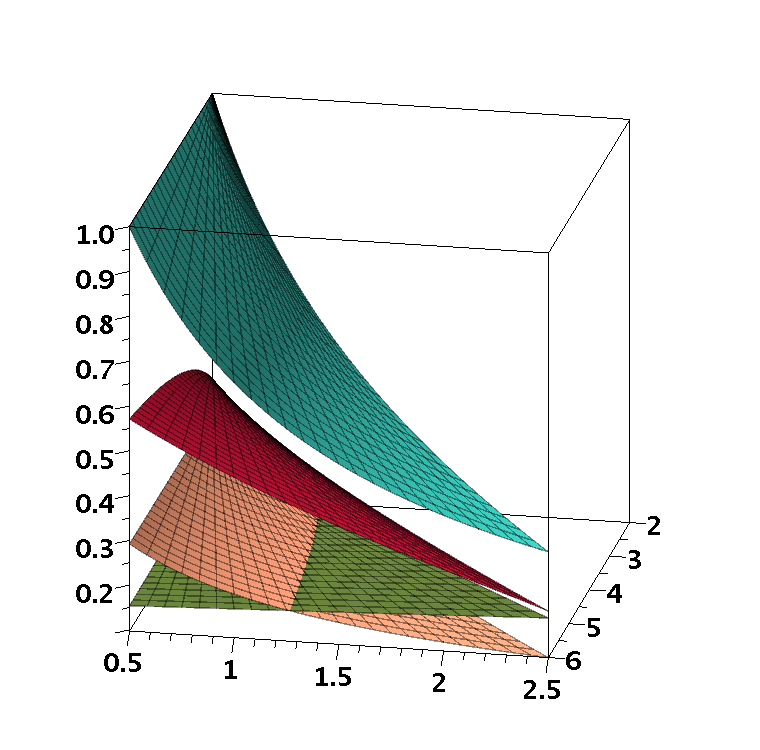
\includegraphics[width=0.95\textwidth, trim={10mm 10mm 10mm 10mm}]{Plots/Plot3dQary}};
		
		\node[draw=none] at (6.5, 1.0) {$\cq$};
		\node[draw=none] at (3.0, 0.05) {$\cg$};
		\node[draw=none] at (.2, 3.05) {$\const$};
		
		\draw[fill=Turquoise, opacity=0.9] (1.2, -0.3) rectangle (1.5, 0.0) node[yshift=-5pt, xshift=14pt]{\scriptsize $\cBKZ=1$};
		
		\draw[fill=Crimson, opacity=0.9] (3.2, -0.3) rectangle (3.5, 0.0) node[yshift=-5pt, xshift=14pt]{\scriptsize Alg.~\ref{alg:ApproxSVP}};
		
		\draw[fill=LightSalmon, opacity=0.9] (1.2, -0.8) rectangle (1.5, -0.5) node[yshift=-5pt, xshift=21pt]{\scriptsize $\cBKZ=0.292$};
		
		\draw[fill=DarkOliveGreen, opacity=0.9] (3.2, -0.8) rectangle (3.5, -0.5) node[yshift=-5pt, xshift=14pt]{\scriptsize Alg.~\ref{alg:ApproxSVPImprived}};
		
		\end{tikzpicture}
	\end{subfigure}
	\begin{subfigure}[t]{0.45\textwidth}
		\centering
		\begin{tikzpicture}
		\node[anchor=south west,inner sep=0] (image) at (0,0) {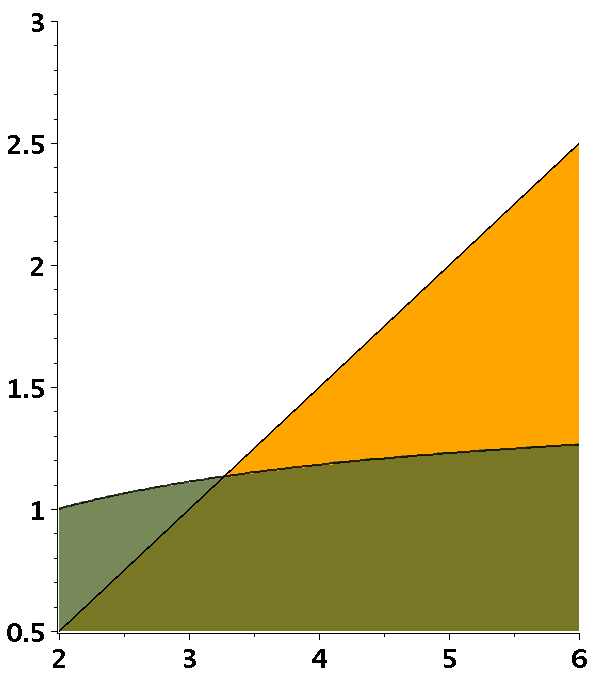
\includegraphics[width=0.80\textwidth, trim={0 0 0 13cm}]{Plots/PlotQAryIneq}};
		
		\node[draw=none] at (-0.01, 3.3) {$\cg$};
		\node[draw=none] at (3.0, -0.1) {$\cq$};
		
		\draw[fill=Orange, opacity=0.9] (0.3, -0.6) rectangle (0.6, -0.3) node[yshift=-5pt, xshift=25pt]{\scriptsize $\cg< \tfrac{\cq}{2} - \tfrac{1}{2}$};
		
		\draw[fill=DarkOliveGreen, opacity=0.9] (2.8, -0.6) rectangle (3.1, -0.3) node[yshift=-5pt, xshift=38pt]{\scriptsize Alg.~\ref{alg:ApproxSVP} $\leq \cBKZ \mkern-3mu=0.292$};
		
		\end{tikzpicture}
	\end{subfigure}
	\caption[Comparison of algorithms for $\appSVP$]{Comparison of two families algorithms for $\appSVP$: those that are based on \BKZ reduction and combinatorial ones. The considered parameter range  is $\cq=[2, \ldots, 6], \cg=[0.5, \ldots \cq/2 - 1/2]$.}
	\label{fig:appSVPCompare}
\end{figure}

\paragraph{Combinatorial \DUAL attack on \LWE.} Recall the \DUAL attack on \LWE with parameters $n, q = \bigO(n^{\cq})$, $\alpha =~ \bigO(n^{-\ca})$ (see Alg.~\ref{alg:Dual} in Sect.~\ref{sec:OtherAttacks}). As the main subroutine, it runs an $\appSVP$ solver on the lattice $\qLATTp(\AMat)$. The approximation factor $\gamma$ depends on the number of \LWE samples provided. Instead of running a $\beta$-\BKZ reduction to solve $\appSVP$ as we do in Sect.~\ref{sec:OtherAttacks}, we can run a combinatorial algorithm for the search of a short vector in $\qLATTp(\AMat)$. In case, we have exponentially-many samples, we run our Alg.~\ref{alg:ApproxSVP} with $\cg = \ca-\cq/2$ in which case the running time of the (combinatorial) \DUAL attack on $\LWE$ is $2^{(\const+\smallo(1))n}$ where $\const = \big(2 \ln\big(\tfrac{\cq}{\cq-\ca} \big) \big)^{-1}$. In case $m=\TLandau(n \log n)$, we resort to the sample amplification which decreases $\ca$ by $1/2$. This results in a smaller approximation factor leading to a worse running time constant $\const = \big(2 \ln\big(\tfrac{\cq}{\cq-\ca+1/2} \big) \big)^{-1}$.
%\subsection{Combinatorial \DUAL and \BKW attacks on \LWE are equivalent} \label{subsec:ReEvalLWE}

In this section we return to the complexity of the Learning with Errors problem -- the question we already addressed in Chap.~\ref{chap:LWEasBDD}. In particular, we re-evaluate the complexity of the \DUAL attack on \LWE described in Sect.~\ref{sec:OtherAttacks} in the light of algorithms for $\appSVP$ presented in previous sections.

Recall briefly the \DUAL attack on \LWE with parameters $n, q = \bigO(n^{\cq}), \alpha = \bigO(n^{-\ca})$. Given $m=2n$ \LWE samples in a matrix form $(\AMat, \bvec = \AMat\transpose \svec + \evec \bmod q) \in \Z_q^{n \times 2n} \times \Z_q^{2n}$, we construct a basis $\DMat$ for the lattice $\qLATTp(\AMat)=\{ \xvec \in \Z_q^{2n} \colon \AMat \xvec = \zerovec \bmod q \}$. It is easy to verify that the matrix given in Eq.~\eqref{eq:BasisD} forms such a basis. The goal of the \DUAL attack is to find a short vector $\vvec \in \qLATTp(\AMat)$, in particular, $\|\vvec \| \leq \bigO(n^{1/2+\ca - \eps})$ for some small $\eps>0$. Once found, we compute $\ScProd{\vvec}{\bvec}$. The result of this inner-product has bias $\delta = 2^{-\bigO(n^{1-\eps})}$, so we can construct a distinguisher (see, for instance, \cite{EC:DucTraVau15} for such a construction) to solve decisional \LWE (see Def.~\ref{def:decLWE}) with success probability $\delta$. In order to use search-to-decision reduction for \LWE \cite{EC:MicPei12}, we boost the success probability of the distinguisher to $1-\smallo(1)$ by finding $\delta^{-2}$-many short $\vvec$'s and verifying $\ScProd{\bvec}{\vvec}$.

In Sect.~\ref{sec:OtherAttacks}, we run a \BKZ reduction algorithm on $\DMat$ to find $\vvec$. The complexity of the \DUAL attack is given in Thm.~\ref{thm:DualSearch} (see also Table~\ref{table:compareTable}). The following simple lemma shows that if instead of \BKW, we use Algorithm~\ref{alg:ApproxSVP} to find $\vvec$, we end up with the complexity that matches the running time of a $\BKW$-type algorithm for \LWE by Guo et al.\ \cite{C:GuoJohSta15} and Kirchner-Fouque \cite{C:KirFou15}. We denote this attack $\DualC$.

\begin{lemma}[\DUAL attack with combinatorial $\appSVP$]\label{lem:LWEDualComb1}
	The \emph{search}-\LWE problem with parameters $(n, q=\bigO(n^{\cq}), \alpha = \bigO(1 / n^{\ca}) )$ where $\cq, \ca = \TLandau(1)$ that satisfy $\ca>\cq/2$, and $m=\Theta(n)$ \LWE samples, can be solved with the $\appSVP$-solver run given in Alg.~\ref{alg:ApproxSVP} in time $T(\DualC) = 2^{(\const+\smallo(1))\cdot n} $, where
	\[
		 \const = \frac{1}{2 \ln \big( \tfrac{\cq}{\cq-\ca} \big) },
	\]
	with $\Psucc(\DualC) = 1- \smallo(1)$.
\end{lemma}

\begin{proof}
	In order to find $\vvec \in \qLATTp(\AMat)$ of length $\| \vvec \| \leq $, we run Algorithm~\ref{alg:ApproxSVP} with the approximation parameter $\cg = $ 
\end{proof}